\chapter{saMsakxqqtAyoVgada parxshAnxvaLige utatxra}

\noindent
{\large\bf saMsakxqqtAyoVgada parxshenxgaLige utatxrisabeVkAda parxkaraNa}\label{page19}
\medskip

\noindent
(saMsakxqqta BASeya vAyxsaMgavananxBivaqdidhxpaDisalu, hiMdomemx saMsakxqqtAyoVgavoMdu keVMdarx sakARradiMda rUpugoMDu, aneVka vidAyxsaMsethxgaLige aBipArxya saMgarxhakAkxgi (AyoVgavu) parxshAnxvaLiyanunx  (parxshAnxvaLiyu saMsakxqqta matutx AMgalx BASeyalilxdudx avugaLanunx anubaMdhada koneyalilx mudirxsalAgide. pu.\Ppageref{questions}) kaLuhisi yoVgayx utatxragaLanunx bayasitutx. A samayadalilx naMjanagUDu tAlUlxku heDatale keSxVtarxdalilx aSATxMgayoVgavijAcnxnamaMdirada keVMdarx kAyARlayavu tananx kAyaRgaLanunx naDesutitxtutx. vijAcnxnamaMdirakUkx  parxshAnxvaLiyu baMdidadxriMda maMdirAdhayxkaSxrAda shirxV shirxVraMga mahAguruvu anugarxhisida viSayagaLanunx (saMsakxqqtiVkarisi) meVlakxMDa AyoVgakekx kaLuhisalAgitutx. adanunx ililx muMdiDalAgide. {\rm 13-02-1956})  
\bigskip

viSaya parxvacana-\hfill leVKana-

shirxVraMga mahAgurugaLiMda \hfill shirxVyuta sheVSAcalashamAR avariMda.

\medskip

\begin{center}
mudarxNakAkxgi pariSakxraNa,\\
shirxVyuta enf. esf. rAmABadArxcArayxriMda. 2-6-1996
\end{center}

\noindent
{\large\bf vidAyxmUlanAda hayagirxVvana samxraNe}\label{page19a}
\medskip

\begin{shloka}
vishovxVtitxVNaRsavxrUpAya cinamxyAnaMdarUpiNeV |\\\label{page19c}
tuBayxM namoV hayagirxVva! vidAyxrAjAya viSaNxveV ||
\end{shloka}

\begin{shloka}
jAcnxnaM teV haMsavijAcnxnamidaM vakASxyXmayxsheVSataH |\\\label{page19b}
yadfjAcnxtAvx neVha BUyoV\char'263 nayxtf jAcnxtavayxmavashiSayxteV ||\\
\hfill Ba. giV
\end{shloka}

\begin{figure}[H]
\centering
{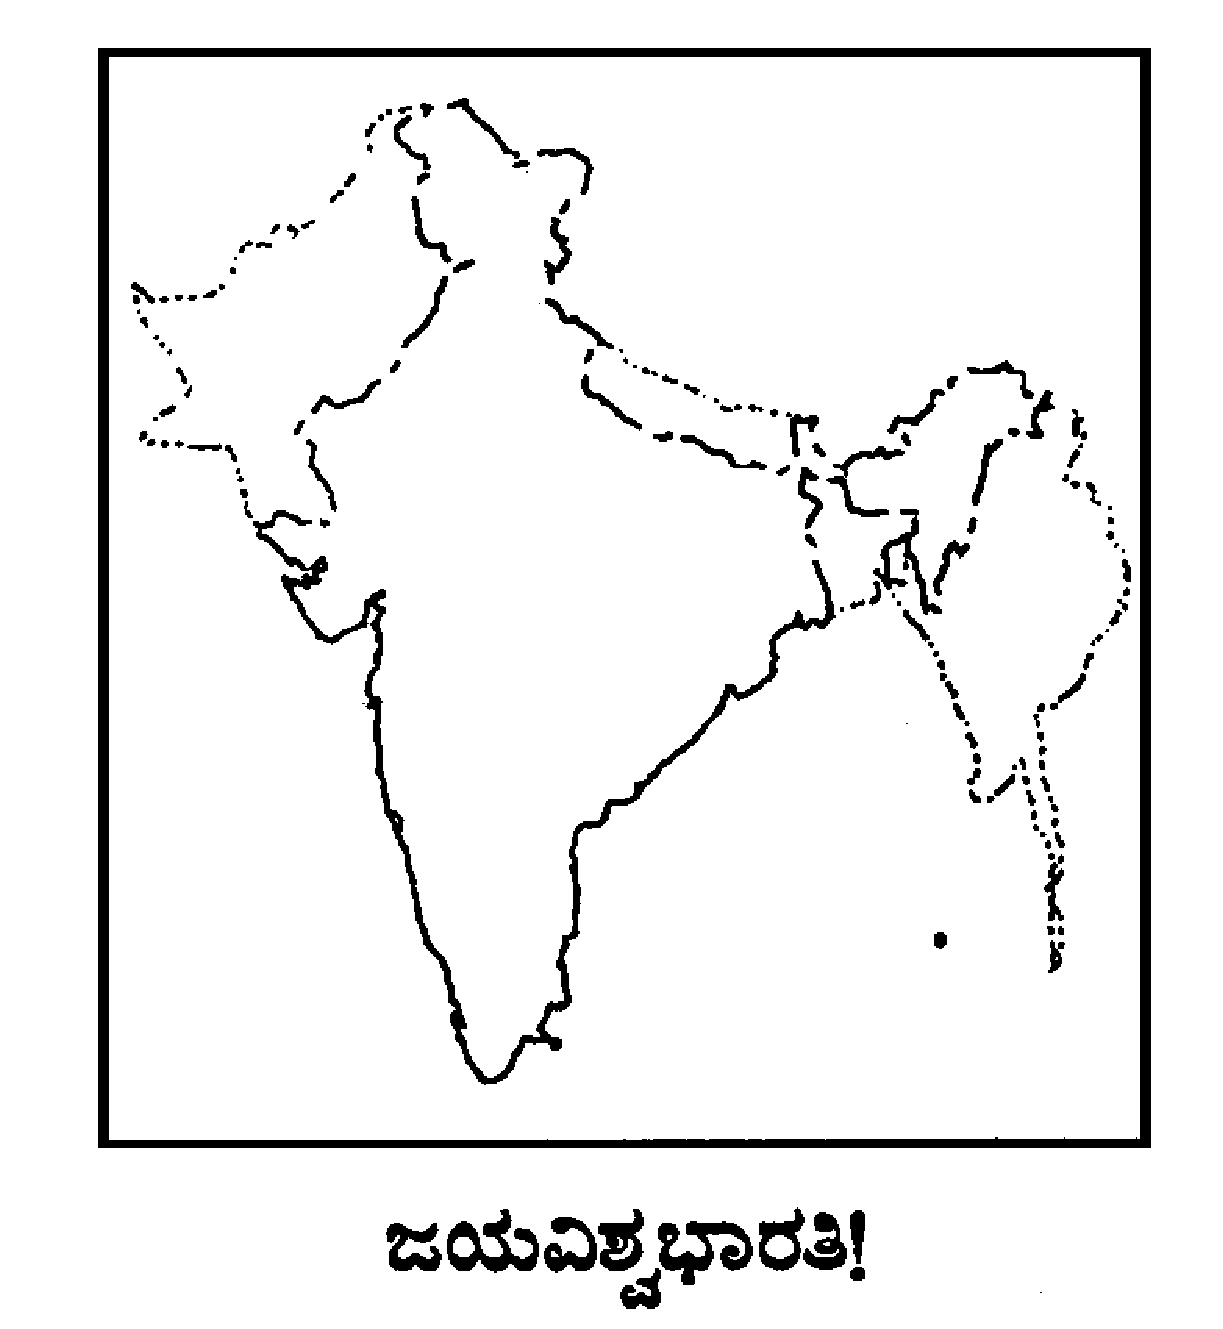
\includegraphics[scale=.19]{0019.eps}}
\caption{jaya vishavxBArati !}
\end{figure}

\noindent
{\large\bf BArata padada athaR vivaraNe}\label{20}
\medskip

\begin{shloka}
BAti saveVRSu veVdeVSu ratiH saveVRSu jaMtuSu |\\\label{20a}
taraNaM savaRtiVthARnAM teVna BAratamucayxteV ||
\end{shloka}

\medskip
\noindent
{\large\bf deVva BASe-saMsakxqqtada baagege shuBAshaMsane}\label{20b}
\medskip

\begin{shloka}
yAvadasitx tarxyiV loVkeV catumuRKamuKoVdaBxvA |\\\label{20c}
yAvadAvx rAmacaritaM vAlikxVki-kavi-citirxtamf ||
\end{shloka}

\begin{shloka}
kaSxraMtayxmaqtadhArA vA yAvadf vAyxsasayx sUkatxyaH |\\
vAgedxVvAyx varaputarxsayx kALidAsasayx vA giraH ||
\end{shloka}

\begin{shloka}
tAvadeVSA deVvaBASA deVviV sAthxsayxti BUtaleV |\\
yAvacacx vaMshoV\char'263 sAtxyXyARNAM tAvadeVSA dhurxvaM dhurxvA ||
\end{shloka}

{\medskip
\noindent
{\large\bf saMsakxqqtAyoVgakekx kaLuhisida viSayagaLa anukarxmaNike}}\label{20d}
\begin{itemize}
\item[{\rm1.}] parxsAtxvane
\item[] utatxragaLu
\item[{\rm 2.}] e. viBAga
\item[{\rm 3.}] bi viBAgada BUmike.
\item[{\rm 4.}] bi viBAgada utatxragaLu.
\item[{\rm 5.}] si viBAga.
\item[{\rm 6.}] Di viBAga.
\item[{\rm 7.}] upasaMhAra
\end{itemize}

{\medskip
\noindent
{\large\bf savaRvidAyxmUlavAda satayxda samxraNarUpavAda maMgaLa}}\label{20e}
\begin{itemize}
 \begin{shloka}
\item[{\rm 1}] IshAnaH savaRvidAyxnAmiVshavxra: savaRBUtAnAmf |\\\label{20f}
barxhAmxdhipati barxRhamxNoV\char'263 dhipati barxRhAmx shivoV meV asutx sadAshivoVmf ||
\item[{\rm 2}] QucoV\char'263 kaSxreV parameV voyxVmanf |\\\label{page21d}
yasimxnf deVvA adhivishevxV niSeVduH |\\
yasatxnanx veVda kimaqcA kariSayxti? |\\
ya itatxdivxdu satx imeV samAsateV ||
\item[{\rm 3}] vijAcnxneVnA\char'263\char'263 tAmxnaM veVdayati |\label{page21g} 
\item[{\rm 4}] na hi jAcnxneVna sadaqshaM pavitarxmiha vidayxteV ||\label{page21f}
 \item[{\rm 5}] QuSiBibaRhudhA giVtaM CaMdoVBiviRvidheY: paqthakf |\\\label{page21e}
barxhamxsUtarxpadeYshecxYva heVtumadiBxviRnishicxteY: ||
\item[{\rm 6}] adhAyxtamxjAcnxna nitayxtavxM tatatxvXjAcnxnAthaRdashaRnamf |\\\label{page21c}
Etatf jAcnxnamiti porxVkatxmf ajAcnxnaM yadayoV\char'263 nayxthA ||
\end{shloka}
\end{itemize}

%~ \begin{itemize}
 %~ \begin{shloka}
 %~ \item[{\rm 5}] QuSiBibaRhudhA giVtaM CaMdoVBiviRvidheY: paqthakf |\\\label{21}
%~ barxhamxsUtarx padeYshecxYva heVtumadiBxviRnishicxteY: ||
%~ \item[{\rm 6}] adhAyxtamx jAcnxna nitayxtavxM tatatxvXjAcnxnAthaRdashaRnamf |\\\label{21}
%~ Etatf jAcnxnamiti porxVkatxM ajAcnxnaM yadayoV\char'263 nayxthA ||
%~ \end{shloka}
%~ \end{itemize}

{\medskip
\noindent
{\large\bf saMsakxqqtAyoVgada kArayxda parxshaMseyoMdige vijAcnxpane}}\label{page21}

\bigskip

{\centerline{\large\bf{shirxV sadugxraveV namaH}}}

\medskip

satayx-jAcnxna-anaMtavAda suKada mUlaneleyAgiruvaMthadAgidadxrU saha, iMdinavarAda namamx kaNiNxniMda dUravAgiruva (daqSiTx goVcaravAgadiruva) sanAtanAyaR BAratiVya saMsakxqqti matutx nAgarikategaLiMda {\rm (Civilization)} samaqdadhxvAgiruva saMsakxqqtaBASeya bagege rASaTxrXda parxjegaLalilx yathAthaRvAda arivu mUDuvaMte mADaloVsuga hoNeyanunx hotutx mahAyajacnxrUpavAda I utatxmavAda kAyaRdalilx kaMkaNabadadhxrAgaliruva saMsakxqqtAyoVgada sadasayxralilx swhAdaRpUNaRvAda vijAcnxpanegaLu.

{\medskip
\noindent
{\large\bf saMsakxqqtada bagegx arivu mUDisuva kArayx nilalxdeV beLeyabeVku}}\label{page21a}
\medskip

\noindent
jiVvanada paramalakaSxyX (guri), adakAkxgi ADikoLuLxva mAtukate, matutx adanunx kirxyeyalilxLisuva naDe ivugaLalilx parasapxra sAmarasayx matutx sAmaMjasayxgaLilalxdaMtAgi, aMdhAnukaraNa paraMpareyalilx sikikxkoMDu muLugutAtx rASiTxrXVya parxjegaLelalxrU adhoVgatiyalilx sAgutatxliruva I desheyalilx, I riVti saMpadaBxritavAda saMsakxqqta BASeya arivu janatege neYjavAgi-satayxvAgi dorakuvaMtAgabeVkeMduMTAgiruva manasusx maraLugADinaMtAgiruvaMtaha I rASiTxrXVya jiVvanadalilx niVrina bugegxyanunx kANuva cihenxyaMte toVruvudAgide. Adare hiVge toVridudx bisilu kudure(maqgamariVcike)yAgibiDadeV, jiVvigaLa jAcnxna pipAseyanunx nijavAgiyU niVgisabalalx ashoVSayxvAda amaqta-jaladhAreyAgi hariyuva jAcnxnagaMgeyAdare mAtarx, BAratiVya parxjegaLa sherxVya: perxVyasusxgaLiMda tuMbida pUNaRjiVvanavu matetx sAdhayxvAdiVtu.

{\medskip
\noindent
{\large\bf BAratiVya videyxkalegaLa guri}}\label{page22}
\medskip

\noindent
namamx deVha, mAtu, manasusx, iMdirxyagaLu, budidhx, parxkaqti matutx Atamx ivelalxkUkx heVge parasapxra atayxMta nikaTavAda saMbaMdhavidudx jiVvanavu naDeyutitxdeyoV, aMteyeV jAcnxna-vijAcnxna cakuSxSakxrAda sanAtanAyaR-BArata mahaSiRgaLu taMdaMtaha, `saMsakxqqti matutx nAgarikate' gaLanonxLagoMDa catuSaSxSiTx(64) videyx (kale)gaLigU matutx vishavxgoVLoVtatxra dhurxvadalilx kUTasathxnAgi beLaguva A paraMjoyxVtisisxgU saha aSeTxV nikaTasaMbaMdhavide. aSeTxV
alalxdeV A videyxgaLelalxvU A paraMjoyxVtiya anuBavada kaDege loVkavanonxyuyxva BAratoVtatxramuKigaLU Agive. {(\rm Mariner's Compass)}

{\medskip
\noindent
{\large\bf vijAcnxnamaMdirada kArayxgaLu hAgu Ashaya}}\label{page22a}
\medskip

\noindent
iMdu kaNamxreyAgiruva aMtaha BAratiVya saMsakxqqti nAgarikategaLa viSayadalilx veYjAcnxnikavAda shoVdhane matutx parxyoVgagaLanunx yathAyoVgayx naDesi, avugaLiMdodagibaMda sAvxnuBavagaLa AdhArada meVle bagege harida viSayagaLanunx avugaLa javAbAdxri, adhikAri, kAla-deVsha-vataRmAnagaLu ivelalxvananxnusarisi, aMteyeV yathAshakitx yathAkAlAvakAsha loVkada muMdiDuvudU vijAcnxna maMdirada AshayavAgide.

{\medskip
\noindent
{\large\bf vijAcnxnamaMdirada hinenxle}}
\medskip

\noindent
keVvala pusatxka pAMDitayxdalilxyeV niMtu, (pusatxkagaLalilx kaMDaMtaha) shAsatxrX vAkayx matutx padagaLanenxV meluku hAkikoLuLxtAtx caviRtacavaRNa mADuvudariMdaleV sanAtanAyaR BAratiVyara shAsatxrXgaLigelAlx EkeYka lakaSxyXvAda badukina (satayxvasutxvina) rasAnuBavavAgadu. A padAthaRda (satayxvasutxvina) jAcnxnAnuBavagaLa beLakinalilx shAsatxrXgaLananxthaRmADikoMDAga tAneV namamx 
savARMgiVNa vikAsarUpavAda A paramashAMtiyanAnxsAvxdisalu sAdhayxvAdiVtu. I KacitavAda aBipArxyavanunx, parxyoVgAtamxkavAda nishacxya hoMdida vijAcnxnamaMdiravu dhiVravANiyiMda heVLahoraTu `na shAmayxti vinApAnaM vAyxdhirwSadhashabadxtaH'\label{25} eMdu daqDhavAgi sArutatxde. (auSadhavanunx pAnamADadeV `auSadhi auSadhi' eMba sadidxniMda mAtarxveV vAyxdhiyu aDagalAradu.)

{\bigskip
\noindent
{\large\bf diviBuvigaLa seVtu-BArata saMsakxqqti}}\label{page23}
\medskip

\noindent
vishavxda saqSiTxge mUlavAdaMtaha A paramashAMtiya tANavanenxV tamamx daqSiTxge neleyanAnxgiTuTxkoMDu (sAdhane mADi), saMpUNaRvAda saqSiTxya meVle oMdu siMhAvaloVkanavanunx biVri, naMtara tamamx manasesxMba rathadalilx kuLitu, diviyiMda BuviyavaregU matetx BuviyiMda diviyavaregU saMcarisi, jAcnxna-vijAcnxnagaLiMda pUNaRrU taqpAtxtamxrU AdaMtha sanAtanAyaR BArata mahaSiRgaLiMda parxkAshagoMDu parxvatiRtavAda saMsakxqqti matutx nAgarikategaLelalxvU, jiVvigaLanunx nirAyAsavAgi aDiDx AtaMkagaLigeDeyilalxdaMte BuviyiMda diviyavaregU koMDoyuyxva oMdu sumAgaRvAgide. A hAdiyanunx nAvu hiDidu horaTare, avaru EpaRDisida A yAnavanunx hatitxdare adu hoVgi talapuveDege nAvU talaputetxVve. adeV jiVvanada neledANavU Agirutatxde. adaralilx oMdu gAMBiVyaRvU swMdayaRvU nitayx swKayxvU iruvudu arivAgutatxde. idu tAtitxvXkavAda sithxti.

{\bigskip
\noindent
{\large\bf `BAratiVya saMsakxqqti' - iMdu gata veYBavada palalxvi}}\label{page23a}
\medskip

\noindent
hiVgiruvalilx I shAshavxtavAda BUmikeyiMda cuyxtiyanunx hoMdi, AdashaRshUnayxvU akaqtayxmayavU Ada sheYshavAvasethxya (neYjavAda ariviniMda dUravAda) modalogxMDu biVLutAtx ELutAtx taDavarisutAtx mugagxrisutAtx dikukxkANadeV gotutxgurigaLilalxdeV Cinanx BinanxvAda kumAgaRgaLiMda tuMbi hoVgiruva iMdina asaMsakxqqtavAda bALATadalilx sanAtanArayx-BArata mahaSiRgaLa saMsakxqqti nAgarikategaLiMdodagatakakx swMdayARnaMdAnuBavavu heVge tAneV sAdhayxvAdiVtu? yAralilx vicArisidarU gataveYBavada palalxviyanunx mAtarx keVLabahudeV horatu sithxtaveYBavakekx elUlx eDeyilalxveMbudu sapxSaTxvAgi tiLiyutatxde.

\newpage

{\medskip
\noindent
{\large\bf ASaR saMsakxqqtiya mamaRvariyadavara vAyxKAyxnagaLa pariNAma}}
\medskip

\noindent
A shAshavxta vasutxvanenxV AdharisikoMDu, adara pArxpitxyanenxV dheyxVyavAgi hoMdi sanAtanAyaR-BArata mahaSiRgaLu parxkAshakekx taMda videyx-kale-shAsatxrX ivugaLigU namamx iMdina bALATada anuBavagaLigU kiMcitAtxdarU sAmarasayxvideyeV? eMbudanunx athaRmADikoLuLxvudU asaMBavavAgide.

BAratiVya saMsakxqqtiyAdarU Enu? eMdu sAvadhAnavAgi shoVdha mADidare, sanAtanAyaR- mahaSiRgaLa keY hiDiyalilx (muSiTx) goVpayxvAgi aDagiruva jiVvamaNiyeV Agiruvudu goVcaravAgutatxde. A QuSimunigaLa muSiTxyalilx EnaDagideyeMbudanunx heVLalu nAnu muMdu tAnu muMdu eMdu horaTavara kUgeV kUgAgideyAdarU, yAra mAtu managaLU vasutxtatatxvXvanunx muTiTx barutitxlalx, matotxMdu pusatxkada mAtananxvalaMbisi hoyodxDutitxdeyeMbudu edudx kANutatxde. avaru tamamx muSiTxyalilx mucicxTuTxkoMDidadxrU, yArAdarU pAradashaRkada mUlaka A mareyanunx teredu (tereyanunx BeVdisi) noVDi toVrisidAga mAtarx A bagegx itarara arivu mUDiVtu. adu horapaTiTxVtu. Adare elalxrU sAruvudU saha taMtamamx bALATadalilx kaMDubaruvudara peYki yAvudAdaroMdanenxV QuSi muSiTxyalalxDagiruva jiVvamaNiyeMdu GoVSiSutAtx kAla yApanemADutitxdAdxre. iMdu A bagegx naDeyuva vAyxKAyxnoVpavAyxKAyxnagaLelalxvU kuruDanige kuruDaneV dAri toVrisa horaTaMtAgide-(aMdheVneYva niVyamAnA yathAMdhAH\label{24})yAdadxriMda IvaRrigU adhoVgatiyeV gatiyAgideyeMdare neYjasaMgatiyadu.

{\medskip
\noindent
{\large\bf yAru mAgaRdashaRkarAgabalalxru?}}
\medskip

\noindent
 AdadxriMda yAru QuSihaqdayavanunx hoMdidavarAgidudx alilxya samAcAravanunx viSaya-parxyoVga matutx anuBavagaLige parasapxra viroVdhavanunx tarada parxyoVga vijAcnxnada baladiMda loVkada muMdiDabalalxroV, avaru mAtarxveV QuSi saMsakxqqti nAgarikategaLuLaLx jiVvanakekx mAgaRdashaRkarAgabalalxreMdu heVLabayasutatxde vijAcnxna maMdira.

{\bigskip
\noindent
{\large\bf BASe-BAvagaLa sAmarasayx}}\label{page24}
\medskip

\noindent
parxkaqta, saMsakxqqta BASeya viSayadalilx eraDu mAtugaLanAnxDabeVkAgide. `BASe' yeMdareVnu? eMba parxshenxge utatxravAgi heVLuvudAdare, BASeyu oDalu-eMdu. oDalige oMdu usiru beVkalAlx eMdare, BAvaveV BASeya usiru. BAvada oDaleV BASe. I riVti BAvakUkx BASegU saMbaMdhavoMdideyeMbudu elalxrU ADikoLuLxvudeVnoV nija. loVkadalilx parxtiyoMdu pArxNiyU tananx oLa BAvavanunx parxkAshapaDisalu nAnAtarahada sAdhanegaLanunx hoMdiruvudu kaMDu barutatxde. hiVgiruvalilx manuSayxnu tananx BAvABivayxkitxgAgi paDediruva aneVka sAdhanegaLa peYki BASeyU oMdu sAdhanavAgide. uLidelalxkikxMta parxmuKavU Agide. BASeyu vayxkatxvAda vAkAkxdare adakekx mUlavu BAvaveV. udAharaNege- roVgiyobabxnu naraLutitxruvudanunx gamanisidare, avana naraLATavU oMdu BASeyenanxbahudu. A BASeyu Enanunx-yAva BAvavanunx horahAkutatxdeyeMdare-oLagina veVdaneyanunx. AdadxriMda naraLATada BASege oLagina veVdaneyeV BAvavAgiruvudu. A veVdaneya BAvavanunx avana naraLuvikeyeV vayxkatxgoLisabalulxdu. yAvudeV mAtanADidarU adariMda A veVdaneyu vayxkatxvAgalAradu. veVdanege hoMdikoLuLxva BASe naraLuvikeyeV. hiVge BASe matutx BAvagaLa sAmarasayxvirabeVku.

{\medskip
\noindent
{\large\bf amara BASe saMsakxqqta}}
\medskip

\noindent
oDalige (deVhakekx) bele usiriniMda heVgoV, hAgeyeV BASege BAvadiMda mAtarxveV beleyiruvudu. I riVti yoVcisi saMsakxqqta BASege belekaTuTxvudAdare, Aga adakekx nijavAda bele. I BASeya BAvavAvudenunxvudAdare-sanAtanAyaR BAratamahaSiRgaLu tamamx susaMsakxqqtavAda aMtaHkaraNadiMda diviyalalxnuBavisida amaraBAvaveV. A amara BAvavanunx vayxkatxpaDisalu-matayxRBUmige taralu baLasida BASeyeV saMsakxqqta BASe. amaraBASe-deVvaBASeyenisikoLaLxlu adara hiMde amara BAvavirabeVku. amara BAvadiMda saMsAkxra hoMdida-pArishudadhxyX hoMdida BASeyeV saMsakxqqta BASe. adu BU-savxgaRgaLeraDanUnx oMdugUDisuva seVtuveyAgide. hiVge BASeya jiVvavAda amaraBAvavanunx kaLedukoMDiruva BASeyAgide iMdu namamx keYge sikikxruva saMsakxqqta BASe. jiVvavanunx kaLedukoMDAga maqtavAguvudaSeTxV. AdadxriMda namamx pAlige dorakiruva BASeyu maqta BASeyAgideyeMdare sariyAgutetx. EkeMdare-iSATxru garxMthasahasarx adhayxyana mADiyU AgutitxruvudeVnu? keVvala pada-vAkayxgaLa cavaRNeyaSeTx. alilxya padAthaRgaLa anuBavavAgaliV adariMda dorakatakakx rasavAgaliV, kiMcitAtxdarU haqdayakekx iLidilalx. iLiyutitxlalx. 

AyaRmahaSiRgaLu tamamx Atamx, manasusx, budidhx matutx iMdirxyagaLalilx yAva AnaMda rasavanunx tuMbikoMDu, A tuMbuneleyAda amaraBAvavanunx, veVda shAsatxrX-purANeVtihAsagaLa rUpavAda yAva saMsakxqqta vANiyalilx gAna mADidaroV, adeV vANiyalilxna veVdashAsAtxrXdi sAhitayxgaLa adhayxyana-adhAyxpanagaLiMda Iga keVvala gaMTalu oNagutitxdeyeV horatu, A AnaMdarasada taMpAgaliV amara BAvavAgaliV namamx pAlige ilalx. hiVgAgalu Enu kAraNa? eMdare iMtaha sAhitayxkArarAda AyaRQuSigaLalilxdadx ASaRvijAcnxnavu namage ilalxdiruvudeV kAraNa. iMtaha duravasethxyalilxdadxrU, bariV duraBimAnavu mAtarx edudx kANutitxde. idelAlx athaRsaMbaMdhavanunx kaLedukoMDa shabAdxDaMbarada veYBava.

{\bigskip
\noindent
{\large\bf BAvadiMda kUDibaMdAga BASege BAvasoVpAnavAguvudu}}\label{page26}
\medskip

\noindent
BagavAnf bAdarAyaNaru athaRdoDane samanavxyavanunx kANada vAkapxrXpaMcadiMda yAvudeV parxyoVjanavU dorakalAradeMdu, mahABAratada shAMti pavaR 244neV adhAyxyadalilx sapxSaTxgoLisidAdxre. niVranunx kuDidAga adara taMpu heVge gaMTalinalilx dorakuvudoV hAge sadABxvavuLaLx vAkayxvanunx samxrisuvudariMdalU A rasavu osaruvudu saMsAkxriyAdavanige eMdiruvaru -

\medskip
\begin{shloka}
BUmisaMsAthxnayoVgeVna vasutxsaMsAthxnayoVgataH |\\\label{26}
rasaBeVdA yathA toVyeV parxkaqtAyxmAtamxnasatxthA ||\\
\end{shloka}

\begin{shloka}
tadAvxkayxsamxraNAninxtayxM taqpitxM vAri pibaninxva |\\
pArxponxVti jAcnxnamaKilaM teVna tatusxKameVdhateV ||\\
\hfill(ma.BA.shAM.pa. sholxV 90-91)
\end{shloka}

himAlayada paramoVnanxta shiKaravAda gwriVshaMkaradalilx odaguva CaLiyu yAva bageyadu? eMdu yArAdarU keVLidAga, sAdhAraNanAda jana, Enu utatxra koDabahudu?  `himAlayadalilx bahaLa CaLi' eMdu avarivara bAyiMda keVLikoMDadadxnUnx, ililx CaLigAladalilx tAnu anuBavisida CaLiyanUnx seVrisikoMDu gwriVshaMkarada CaLiyanunx vaNiRsahoraTare, avana BASeyalilx avana dhavxniyalilx yAva CaLiyu vayxkatxvAdiVtu! eMdu Uhisabahudu. avana anuBavagoVcaravAdudu vayxkatxvAgabahudeV horatu gwriVshaMkaradadxlalx. Eke? avana mAtina hiMdugaDe A BAvavilalx. BAvarahitavAda BASe. athavA salalxda beVre bageya BAvadiMda kUDikoMDa BASe. adu nijAMshada kaDege namamxnunx oyayxvudilalx. avana aMtaraMgavanunx muTiTxlalx. `himAlayada ututxMga shiKarada CaLi' eMdu bAyiMda vaNaRgaLanunxcacxrisidarU, adara hiMdina BAva namamx parisaradedxV Agide. inunx alilxgeV hoVgi A CaLiyanenxV PiVlf mADi adara nenapu meYyalilx adara tanadoMdige uLididudx, A bagegx heVLidAdxdare A BAvavanunx A BASeyiMda matotxbabxrige talapisabahudu. hAge heVLalu adakakxnuguNavAda manoVdhamaRvU beVku. adakekx takakx deVha dhamaRvU beVku. hAgidAdxga mAtarx adara ucAcxraNeyiMda savxlapx paricaya dorakabahudu. A CaLiya neYjavAda anuBavaveMdare elAlx iMdirxyagaLa nishecxVSaTxvAda oMdu vicitarx sithxti. A sithxtiyanunx namamx BASeya mUlaka vayxkatxgoLisabeVkAdare adaralilx yAva veYshiSaTxyXvirabeVku? gwriVshaMkarada CaLiyeMdu mAtarx heVLidare sAladu.

{\bigskip
\noindent
{\large\bf saMsakxqqta BASAdhayxyana yAvAga sAthaRka?}}\label{page27}
\medskip

\noindent
aMteyeV A jAcnxnameVrugiriya tudiyanenxVri, alilx amara BAvavananxnuBavisida AyaR-mahaSiRgaLu, A amaraBAvada divAyxnuBavavanunx adakakxnuguNavAda manoVdhamaRdiMda susaMsakxqqtavAda vANiya mUlaka hADidAdxre. avara manoV dhamaRvanunx hoMdi avaraMteyeV saMsakxqqta vANiyalilx gAnamADuvaMtAdare mAtarx, adu namamx pAlige namamx muMdina piVLigege amaravANiyAgabalulxdu. AyaRmahaSiRgaLa gurukuladiMda baMda shikaSxNa rakaSxNagaLu iMdu namage dorakada kAraNa, parxyoVga
vijAcnxnavu lupatxvAgi amara BAvavilalxda vANiyAgi, `mara' vANiyAgi, amara sAhitayxgaLelAlx virUpa hoMdirutatxve. matetx adu savxrUpa hoMdabeVkAdare nAvu amara BAvakekxVrabeVku. anaMtara nAvu baLasuva BASeyu deVva BASe-saMsakxqqta BASeyAdiVtu. hAgAdare mAtarx A BASeya adhayxyanavu sAthaRkavAdiVtu.

{\bigskip
\noindent
{\large\bf visAtxravAda parxsAtxvaneya agatayx}}\label{page27a}
\medskip

\noindent
AyaR mahaSiRgaLa saMsakxqqti - nAgarikate - BASe ivugaLa bagegx iSuTxhiridAda parxsAtxvaneyeVke? eMdare-deYviV manavananxvalaMbisidadx mahaSiRgaLu, adhayxyana matutx adhAyxpanagaLu sariyAda dheyxVyoVdedxVshagaLoDane sAgalu yoVjane hAkidAdxraSeTx ! avara deYviVmana hoMdida dheyxVyoVdedxVshapUNaRvAda shikaSxNa padadhxtiyeV sherxVyaH perxVyasusxgaLige sAdhanavAdudu-eMbudanunx saMsakxqqtAyoVga sadasayxra nenapige taraloVsuga-eMbudu adara utatxravAgide.

{\bigskip
\noindent
{\large\bf ASaR hAgu sAMparxtika shikaSxNa padadhxtigaLalilx ajagajAMtara}}\label{page28}
\medskip

\noindent
iMdu vidAyxBAyxsaveMdu hesarisi horaTu mADutitxruva shikaSxNa padadhxtigU AyaRmahaSiRgaLa shikaSxNa padadhxtigU dakiSxNa dhurxva utatxra dhurxvagaLigiruvaSuTx aMtaravuMTAgide. EkeMdare avara AraMBa dheyxVya matutx karxmagaLigU, namamxlilx Iga naDeyutitxruva vidhAnada AraMBa, dheyxVya matutx karxmagaLigU kiMcitUtx saMbaMdhavilalxvAgide. jiVvanadalilx sAdhisabeVkAda aMshagaLanunx aMdare, dhamaR-athaR-kAma-matutx moVkaSxgaLanunx-nAlUkx puruSAthaRgaLanUnx karxmabadadhxvAgi viBAgisikoMDu, modalaneyadAda dhamaR koneyadAda moVkaSx ivugaLa meVregaLanunx miVradiruvaMte madhayxda athaRkAmagaLeraDanUnx aLavaDisi, deVheVMdirxyagaLa suKarUpavAda perxVyasasxnUnx AtAmxnaMda rUpavAda sherxVyasasxnUnx sAdhisalu anukUlavAgatakakx jiVvana nivaRhaNege beVkAda shikaSxNa karxmavu pArxciVnarAda vidAyxBAyxsa parxvataRkara guriyAgitutx matutx padadhxtiyAgitutx. iMdina padadhxtiyalilx vidAyxBAyxsada pArxraMBa matutx payaRvasAnagaLalilx hoMdANikeyilalxdeV, sadAshayavU ilalxdeV, yAradoV aMdhAnukaraNadalilx sAgutitxruvudariMda parxcaCxnanxvAgiyU parxkaTavAgiyU udarada beLavaNigeyeV muKayxvAgidudx mahaSiRgaLa sharxmavu mUleVpAlAgiruvudu sAvadhAnavAgi noVDuvavarigU parxtayxkaSxveVdayxvAgide.

I bagegx amara kaviyAda kALidAsanu amara sAhitayxdalilxyeV raGurAjana jiVvanavanunx citirxsutAtx AyaRBAratiVyara jiVvana padadhxtiya Adi-madhayx-aMtayxgaLanunx heVge namamx muMdiTiTxdAdxneMbudanunx kANabahudu.

\medskip
\begin{shloka}
sheYshaveV\char'263 BayxsatxvidAyxnAM ywvaneV viSayeYSiNAmf |\\\label{28}
vAdhaRkeV munivaqtitxVnAM yoVgeVnAMteV tanutayxjAmf ||\\
\hfill (raGuvaMsha) - 1:8
\end{shloka}

I tarahada jiVvanavayxvasethxyanunx parxtiyobabx BAratiVya parxjeyalUlx rakatxgatavAguvaMte mADi beLesuva padadhxtiyeV saMsakxqqta vidAyxBAyxsa padadhxtiyeMbudanunx mareyuvaMtilalx.

{\bigskip
\noindent
{\large\bf saMsakxqqtAyoVgada sadAshayada bagegx aBinaMdane}}\label{page29b}
\medskip

\noindent
pArxciVna padadhxtiyanUnx navayx padadhxtiyanUnx tulanAtamxkavAgi AmUlAgarx noVDi navayxpadadhxtiyiMdodagiruva piDuganunx dUramADi pArxciVna vidAyxBAyxsa padadhxtiyanenxV namamx rASaTxrXdalilx punaH anuSAThxnakekx taMdu, saMsakxqqta vidAyxBAyxsada neYjavAda sobaganunx BAratadalilx maraLi saviyuvaMte mADabeVkeMba
AshayadiMda horaTu, A satAkxyaRdalilx badadhx diVkaSxrAgiruva saMsakxqqtAyoVgada sadasayx vaqMdakekx, KAsagiV saMsethxyAgidudxkoMDu videyxgaLa bagege veYjAcnxnika daqSiTxkoVnadiMda ciMtana maMthana kArayxgaLalilx toDagiruva vijAcnxnamaMdiravu aBinaMdanegaLananxpiRsutatxde.

{\bigskip
\noindent
{\large\bf saMsakxqqtAyoVgada parxshenxgaLa kuritu}}\label{page29}
\medskip

\noindent
meVlakxMDa saMsakxqqtAyoVgada sadasayx maMDalige vijAcnxna maMdirada viLAsavu heVge tiLiyiteMbudu namamx arivige baMdilalxvAgide. AdarU saMsakxqqtAyoVgadiMda saMsakxqqta vidAyxBAyxsada bagege parxshAnxvaLiyoMdu bahaLa vilaMbavAgi vijAcnxna maMdirakekx talapide. meVle heVLida parxshAnxvaLiyalilx kANuva kelavu parxshenxgaLu punarukatxvAgiruvudu kaMDubarutetx. inUnx kelavu parxshenxgaLu aMki aMshagaLige saMbaMdhapaTiTxruvudariMdalU, A aMki aMshagaLanunx vijAcnxna maMdiravu saMgarxhisiTuTxkoMDilalxvAdadxriMdalU, matetx kelavu parxshenxgaLige sadayxda parisithxtiganuguNavAgi utatxragaLanunx horagiDalu maMdiravu saMkalipxsilalxvAdadxriMdalU, laBisida kAlAvakAshadalilx kelavu parxshenxgaLige mAtarx utatxragaLanunx kaLuhisutitxde.

{\bigskip
\noindent
{\large\bf vijAcnxna maMdirada I BUmikeyanunx hinenxleyoMdige parishiVlisuva bagege vijAcnxpane}}\label{page29a}
\medskip

\noindent
saMsakxqqti-nAgarikate-saMsakxqqta BASe matutx shAsatxrXgaLa saMbaMdhiyAda parxshenxgaLige, I modaleV tiLisiruvaMte, veYjAcnxnikavAda shoVdhane matutx parxyoVgagaLiMdodagida sAvxnuBavada AdhArada meVle bageharida viSayagaLanunx, AyA viSayagaLa javAbAdxri-adhikAra matutx kAladeVsha - vataRmAnagaLananxnusarisi yathAshakitx loVkada muMdiDuva Ashaya hoMdida vijAcnxna maMdirada kaDeyiMda, viSaya-parxyoVga-anuBavagaLa parasapxra viroVdhakekxDegoDada sAmarasayx-sAmaMjasayxgaLanonxLagoMDa, parxyoVga vijAcnxnada beLakinalilx rUpugoMDa utatxragaLAgive ivu. aucitayxvarita parxyoVga vijAcnxnada daqSiTxyiMda, I BUmikeyanUnx matutx utatxragaLanUnx parishiVlisi manavarike mADikoLaLxbeVkAda javAbAdxriyu, idanonxVduvavarigirabeVkeMdu swhAdaRdiMda vijAcnxna maMdiravu vijAcnxpisutatxde.

{\bigskip
\noindent
{\large\bf patarxvayxvahAradiMda viSayada pUNaR paricaya sAdhayxvilalx}}\label{page30e}
\medskip

\noindent
AyaR BAratiVyariMda horabaMda shAsatxrX-videyx matutx kalegaLa amaraBAvavu keVvala garxMtha rAshigaLa paThana-raTanagaLiMda loVkada anuBavakekx barutitxlalxvAgi, vicAra matutx parxyoVgagaLa sAmarasayxvanunx kApADuva udedxVshadiMda, anuBava sidadhxvAda elAlx aMshagaLanUnx patarx vayxvahArada mUlaka parxcAra mADuva kAyaRkarxmavanunx vijAcnxnamaMdiravu iTuTxkoMDilalxveMdu tiLisutitxdedxVve.

{\bigskip
\noindent
{\large\bf utatxragaLu:-}}
\medskip

\noindent
e. sAmAnayxBAga-

kelavu mUlaBUta parxshenxgaLu matutx avugaLa utatxragaLu.

(vi.sU:- parxshenxgaLa saMKeyxyanunx mAtarx nideVRshisi, utatxragaLanunx baredide.)

{\bigskip
\noindent
{\large\bf saMsakxqqtajacnxna vishiSaTx pAtarx}}\label{page30a}
\medskip

\noindent
(1) sanAtanAyaRBArata mahaSiRgaLiMda parxkAshitavAgi parxvatiRtavAda saMsakxqqti - nAgarikate matutx saMsakxqqta BASegaLalilx yathAthaRvAda(toVrikege siVmitavAgada) anuBavavanunx paDedu, adanunx vishavxBAratada rASiTxrXVya jiVvanadalilx beLakige taruvudeV (tiroVhitavAgiruvudanunx puroVhitavAgi mADuvudeV) saMsakxqqtajacnxnenisikoLuLxvavanu vahisabeVkAda vishiSaTx pAtarxvAgide.

{\bigskip
\noindent
{\large\bf rASaTxrXdalelxV saMsakxqqta BASege gwrava mayARdegaLu salulxtitxlalx}}\label{page30b}
\medskip

\noindent
(2-e) \\yAva oMdu amara BAva matutx QuSimanoVdhamaRvanunx tananx usiranAnxgi mADikoMDu saMsakxqqta BASeyu Buvige iLidu baMtoV, A amaraBAva-QuSimanoVdhamaRgaLu iMdina janateya pAligilalxvAgiruvudariMda, namamx pArxMtadalelxV Eke? samagarx rASaTxrXdalelxV saMsakxqqta BASege ucitavAda gwrava mayARdegaLu salulxtitxlalx. aMteyeV A bagegx yathAthaRvAda sharxdAdhx pirxVtigaLU kaMDu barutitxlalx.

{\bigskip
\noindent
{\large\bf BASeya puroVBivaqdidhxge beVkAda kArayxyoVjanegaLa aBAva}}\label{page31}
\medskip

\noindent
(2-bi) \\ pAThashAlegaLu, mahAvidAyxlayagaLu matutx vishavx vidAyxlayagaLalUlx, Adhunika riVtiyanunx keYgoMDu naDeyutitxruva saMsakxqqtABAyxsavaSuTx mAtarxvalalxdeV saMsakxqqta sAhitayx matutx adaradedxV saMsakxqqtigaLa puroVBivaqdidhxya bagege naDeyabeVkAda kAyaRgaLAgaliV adakekx yoVgayxvAda vayxvasethxyAgaliV yAvudU pArxmANikavAgi rUpugoMDilalxvAgide.

{\bigskip
\noindent
{\large\bf saMsakxqqta BASe hAgU sAhitayxgaLa vAsatxvika aBivaqdidhx}}\label{page31a}
\medskip

\noindent
AyaRmahaSiRgaLa amaraBAvada oDalenisuva saMsakxqqta BASeya kAluBAgadaSaTxkikxMtalU savxlapxvAda aMsha mAtarxveV namage goVcaravAguva saMsakxqqta BASeyAgide. uLida mukAkxlu BAgakikxMtalU adhikavAda BAgavu QuSihaqdayadalelxV gUDhavAgi aDagikoMDide. idanunx shurxtiyeV sapxSaTxmADide.

\smallskip
\begin{shloka}
catAvxri vAkapxrimitA padAni | tAni vidubArxRhamxNA yeV maniVSiNaH |\\\label{31}
guhA tirxVNi nihitA neVMgayaMti | turiVyaM vAcoV manuSAyx vadaMti ||
\end{shloka}
\smallskip

eMbudAgi. aMtaha QuSi haqdayavanunx hokukx adanunx parxkAshakekx taMdu loVkakekx paricaya mADikoTaTxre mAtarx, adara bagegx yathAthaRvAda sharxdedhxyu beLediVtu. I riVti tiLisidaMtaha saMsakxqqta BASeya vayxkAtxvayxkatx sithxtiyanunx anuBavakekx taMdukoLuLxvudeV saMsakxqqta BASe matutx saMsakxqqta sAhitayxgaLa vAsatxvikavAda aBivaqdidhxyAgide.

\newpage

{\bigskip
\noindent
{\large\bf saMsakxqqtada viSayadalilx neYjavAda sharxdedhx beLesuva upAya}}\label{page31b}
\medskip

\noindent
(3-e)\\ 
saMsakxqqta BASA sAhitayxgaLalalxDagiruva mAnava jiVvanada tatatxvXgaLu matutx saMsakxqqti ivugaLalilx parxyoVga vijAcnxnada daqSiTxyanunx hariyisi adariMda anuBavakekx taMdukoMDu pariNata-parxjacnxrAdavaru BArata gaNarAjayxda parxjegaLa manasisxnalilx parishudadhxvAda saMsAkxravuMTAguvaMte mADidare, saMsakxqqtada viSayadalilx neYjavAda paricaya matutx sharxdedhxgaLu beLeyuvaMtAdiVtu.

{\bigskip
\noindent
{\large\bf sAhitayx akADamiya kuritu}}\label{page30d}
\medskip

\noindent
(3-bi)\\ 
sAhitayx akADemiya nidiRSaTx kAyaRkarxmagaLa bagege paricayavu vijAcnxna maMdirakekx bAradiruva kAraNa, A akADemiyu saMsakxqqtAdhayxyanada viSayadalilx yAva riVti Adara sharxdedhxgaLanunx hoMdi saMsakxqqta sAhitAyxBivaqdidhxge neravAdiVteMdu heVLuvudu asAdhayxvAgide.

{\bigskip
\noindent
{\large\bf ASaRgarxMthagaLa BASAMtaravanunx kuritu}}\label{page30c}
\medskip

\noindent
iMdina sAmAjika parisithxtiyalilx ASaRgarxMthagaLu mAtarxveV saMsakxqqtABAyxsakekx poVSakavAgiruvudariMda, A ASaRgarxMthagaLanunx iMgilxVSu matutx pArxMtiVya BASegaLa athARnuvAdadoDaneV utakxqqSaTxvAda riVtiyalilx mudirxsi parxkAshapaDisi saravxrigU sulaBavAgi dorakuvaMte mADabeVkAgiruvudu ucitaveMdu toVrutatxde. aMteyeV ASaRgarxMthagaLalalxDagiruva deYviV BAvavanunx haqdayakekx TArxnfsxleVTf mADi taNisabeVku. ilalxdidadxre bariV daNivu Odugarige. 

{\bigskip
\noindent
{\large\bf BAratiVya saMsakxqqta-saMsakxqqtiya are paricaya apAyakAri}}\label{page30}
\medskip

\noindent
(4-e)\\ 
BArata deVshada vidAyxsaMsethxyiMda utitxVNaRnAda yuvakaneMdAdameVle BAratiVyavAda saMsakxqqta-saMsakxqqtiya alApxlapxparicayamAtarxvidadxre sAladu. pUNaRparicayaveV irabeVkAdudu atAyxvashayxka. EkeMdare ivanunx tananx alApxlapx paricayavanunx itararige koDalu horaTAga samagarxnoVTa dorakadeV matetx vikaqta rUpavanenxV tALiVtu.

\smallskip
\noindent
(4-bi)\\ 
aMteyeV paradeVshagaLalilx hoVgi kaliyuva BAratiVya vidAyxthiRgaLAgaliV, rAjakiVyAdhikArigaLAgaliV, BAratiVya saMsethxgaLa kAyaRkataRrAgaliV, horaginavarige I sanAtanAyaR BAratiVya saMsakxqqtiya nijavAda paricayavanunx koDuvaMthavarAgabeVkAdare, modalu saMsakxqqtiya mUlavananxritavarAgabeVku. ilalxdidadxre I saMsakxqqtiya yathAthaRvAda paricayavanunx koDalAguvudilalx.

{\bigskip
\noindent
{\large\bf mamaRjacnxrAda saMsakxqqta vidAvxMsara niyoVjane}}\label{page32}
\medskip

\noindent
(4-si)\\ 
I AyaRBArata QuSigaLa saMsakxqqtiya mamaRvarita saMsakxqqta vidAvxMsarugaLanunx videVshagaLalilxruva BAratada rAyaBAri kaCeVrigaLalilx niyoVjisidedxV Adare AyA rAyaBAri kaCeVrigaLalilx niyoVjisidadxriMda alilx AgabeVkAda sAMsakxqqtika kArayxgaLu sugamavAgi naDeyalu anukUlavAguvudu. ilalxdidAdxga saMsakxqqtiya apaparxcArakekx kAraNavAdiVtu.

{\bigskip
\noindent
{\large\bf saMsakxqqta BASeya sAvaRtirxkavAda baLakeya kuritu maMdirada niluvu}}\label{page33g}
\medskip

\noindent
(5)\\ 
Iga saMsakxqqta BASeyu iMtaha vAyxvahArika vAyxpitxyanunx hoMdadeV iruva kAraNa, parxkaqta I hiMde sUcisida saMdaBaRgaLalilx saMsakxqqtavanunx baLasuvudu asAdhayxveMdeV toVrutatxde. hiVgiruvudAdarU keVvala cApalayxkokxLapaTuTx saMsakxqqtavanunx baLasidedxV Adare, BASeyalilx athaRciMtaneyAgaliV, BAvAnuguNavAda dhavxniyAgaliV, seVrikoLaLxdeV keVvala BASA shabadxgaLa kaMThapATha mAtarxvAgi uLiyuvaMtAgutatxde. I riVti athaRhiVnavAgi nilulxvaMte mADuvudakikxMtalU, sulaBavAgi athaRvAgutitxruvaMtaha beVre yAvudeV BASeyalelxV AdarU susaMsakxqqtavAda manoVBAvavanunx vayxkatxgoLisuva kAyaRvu Igegx savaRsherxVyasakxraveMbudu namamx aBipArxyavAgideyeMdu heVLabayasutetx vijAcnxna maMdira.
\medskip

\noindent
(parxshAnxvaLiyalilxruva 6neV parxshenxge anugarxhisirabahudAda utatxra laBayxvilalx)

{\bigskip
\noindent
{\large\bf saMsakxqqta BASeya ucAcxraNeyu rASATxrXdayxMta EkarUpavAgabahudeV?}}\label{page33a}
\medskip

\noindent
(7-e)\\ 
rASaTxrXda elAlx pArxMtagaLalUlx janaru oMdeV bageyalilx saMsakxqqta BASeyanunxcacxrisuvaMte mADuvudaMtU asAdhayxvAda kAyaRveV sari. EkeMdare-BASeya ucAcxraNeyu, Binanx BinanxvAda BwgoVLika parisithxtigaLanUnx, janara AhAra-vihAra-vayxvahAragaLanUnx, deVhadhamaR matutx manoVdhamaRgaLanUnx avalaMbisiyeV rUpugoMDiruvudu nishicxtavAdudariMda, adelAlx EkarUpatege baralu sAdhayxvAdAga mAtarx AgabahudAdudanunx avugaLalAlxva badalAvaNeyU ilalxdeyeV EkarUpa mADabayasuvudu parxyoVjanakAriyeV alalx. anukaraNeya sAmathayxRvanunx alalxlelxV huDuki kelavu janaralilx savxlapxmaTiTxna EkarUpateyanunx taruvudu sAdhayxvAdiVtAdarU Agabahudu. EneV AdarU bahaLakAla adaralilx pArxdeVshikateya vAsaneyu idedxV iruvudu.

\newpage

{\bigskip
\noindent
{\large\bf saMsakxqqtakekx pArxdeVshika BASAlipigiMtalU deVvanAgariVlipiya anavxyavu upayukatx}}\label{page33f}
\medskip

\noindent
(7-bi)\\ 
saMsakxqqta BASege hoMdikoLuLxva lipi (baravaNige)yu yAvudAdiVtu? yAvataraha iruvudu yoVgayx? matutx Iga rUDhiyalilxruva deVvanAgariVlipiyu AyaRmahaSiRgaLa saMsakxqqta saMsakxqqtigaLige hoMdikoLuLxva taraha veYjAcnxnikateyuLaLxdedxV? alalxveV? eMba aMshavanenxlAlx tiLiyalu shAsitxrXVyavU veYjAcnxnikavU Ada saMshoVdhaneyu naDeyabeVkAguvudu. AdarU iMdu pArxMtiVyavAgi vividharUpa tALiruva beVre beVre lipigaLu saMsakxqqta BASeya elAlx vaNaRgaLigU saMkeVtavAgalu beVkAda pUNaRteyanunx hoMdadeV iruvudariMdalU, deVvanAgariV lipiyu IgAgaleV elAlx kaDeyalUlx hecucx parxcAra paDediruvudariMdalU, saMsakxqqta garxMthagaLanunx AyA pArxMtiVya lipiyalilx baredare, deVshada itara BAgagaLalilxya janarige athaRmADikoLuLxvudu asAdhayxvAdudariMdalU, tatAkxlakekx saMsakxqqta
BASeya leVKana matutx mudarxNa kArayxgaLige deVvanAgariV lipiyoMdanenxV rASaTxrXdalelxlAlx upayoVgisuvudu saMsakxqqta vidAyxBAyxsada aBivaqdidhxge sahAyakaraveV Aguvudu. 

deVvanAgariV lipiyalalxlalxdeV AyA pArxMtiVya lipiyalilx baraha matutx \hbox{mudarxNa} hoMdiruvaMtaha upayukatxvAda aneVka saMsakxqqta BASA garxMthagaLu deVvanAgariV lipiyalilx mudirxtavAgi parxkAshakekx baMdidedxV Adare deVshiVyarAda elAlx janarigU upakAravAgutatxde. I kArayxvanunx nivaRhisalu parxcArakarige pArxdeVshika lipigaLa paricayavU atayxMtAvashayxkavAgutatxde. pArxdeVshika BASegaLige saMsakxqqta BASegU anoyxVnayx saMbaMdhavanUnx, pArxMtiVya janara saMsakxqqta BASA paricayavanUnx daqDhiVkarisalu, keVvala pArxMtiVyalipigaLu (baMgAli-telugu-kananxDa) itAyxdi tAtAkxlikavAgi anUkUlaveMdu toVridarU, samagarx deVshada daqSiTxyiMda aSeTxVnU lABadAyakavAgadeMdu toVrutetx.

{\bigskip
\noindent
{\large\bf BASege vAyxkaraNavoMdanunx nimiRsuvudara paramoVdedxVshayx}}\label{page34}
\medskip

\noindent
(7-si)\\ 
AyAkAlavanunx parxtinidhisuvaMtha garxMthagaLanunx parishiVlisalAgi, saMsakxqqta BASeyu QuSigaLa kAladiMda pArxraMBisi, janara AcAra vicAragaLu vihAra vayxvahAragaLu kAladeVshagaLu matutx parisithxtigaLananxnusarisi mApaRDutAtx baMdiruvaMtaha naDeyu kANabarutatxde. aSeTxV alalxdeV I saMsakxqqta BASeya vayxvasethxgAgi oMBatutx vAyxkaraNagaLu parxvaqtatxvAdudu kaMDubaMdide. BASege vAyxkaraNavoMdanunx nimiRsuvudara paramoVdedxVshayxvAdarU enu? eMbudAgi 
sUkaSxmXvAgi parishiVlisidare, keVvala perxVyasisxnalelxV (aihika suKamAtarx) mukAtxyagoLaLxliruva bALATavanunx sherxVyoVmayavAgi (pAratirxka suKa) mADi, vAknamxyada mUlavanunx nenapige taruvaMtaha BASA vayxvahAravanunx loVkadalelxVpaRDisuvudeV, eMdu nishicxtavAgutatxde. EkeMdare-vAkikxna vAyxpitxyu parxkaqtiyiMda hiDidu AtamxdavarevigU iruvudAgide. manuSayxna elAlx horavayxvahAragaLU manasasxnenxV mUlavAgi hoMdirutatxve. AdadxriMda-avanavana manasasxnanxnusarisiyeV avanavana AkAra-veVSa-BUSaNa elalxvU EpaRDuvudeMdu loVkaviditavAgide. I AkArAdigaLa mUlaka, `avana manasusx iMtahudeV' eMdu kushalanAdavanu tiLiyabahudu. idaraMteyeV vAknmxya mUlakekx takakxMteyeV BASegU hora AkAravu irabeVkAdudu neYsagiRkavAgide. BASege iMtaha mUlakekx anuguNavAda AkAravanunx kalipxsuvudeV vAyxkaraNada paramoVdedxVshayxvAdudeMbudu, vAyxkaraNavanunx veYjAcnxnika daqSiTxyiMda parishiVlisidAga sidadhxvAguva viSaya.

{\bigskip
\noindent
{\large\bf saMsakxqqtada saraLiVkaraNa kuritu maMdirada niluvu}}\label{page35}
\medskip

\noindent
iMtaha ASaRvijAcnxnaveYBavadiMda rUpugoMDa pANini mahaSiRgaLa vAyxkaraNavu, veYdika matutx vAyxvahArikavenisuva saMsakxqqta vAknmxyada suvayxvasethxyanunx rUpisutitxde. pANini mahaSiRgaLiMda rUpisalapxTaTx I vijAcnxnada beLakinalilx-pArxciVna matutx Adhunika kAlada dhAmiRka-rAjaneYtika-sAmAjika matutx AthiRka keSxVtarxgaLanunx sUkaSxmXmatiyiMda parishiVlisi,

\begin{shloka}
EkaH shabadxH samayxkf jAcnxtaH suSuThx parxyukatxH savxgeVR loVkeV kAmadhugaBxvati\label{35}
\end{shloka}

eMbudAgi ciMtisidaMtaha BASA vayxvahAravu rUDhige baruvaMte mADabeVku. idanenxV vijAcnxna maMdiravu saMsakxqqtada saraliVkaraNa{(\rm Simplification)} athavA pArxthamikavAda saMsakxqqtada vikAsaveMdu aBipArxya paDutatxde. saMsakxqqta vidAvxMsarenisikoMDavaru ASaRvijAcnxnavanunx meYgUDisikoMDu I kelasavanunx nivaRhisabeVkAguvudeMdu vijAcnxna maMdiravu sUcisutatxde.

(7-Di)\\ 
saMsakxqqta BASeyu veYjAcnxnikavAgi beLedu baMdiruvudariMda adanunx namamx parxyatanxdiMda saraLagoLisabeVkAda avashayxkateyeVnU  iruvudilalx. saraLagoLisa horaTu vikaqta rUpavanunxMTumADidare, saMsakxqqta BASe, saMsakxqqta sAhitayx matutx I BASeya hiMdiruva vijAcnxna ivelalxkUkx AGAtavAgutatxde.

{\medskip
\noindent
{\large\bf vidAyxBAyxsa hAgU sAvaRjanika vayxvahAra keSxVtarxkekx saMsakxqqtada anavxya-utatxma}}\label{page36}
\smallskip

\noindent
(8-e)\\ 
AyA pArxMtayxgaLalilxyU, vidAyxBAyxsa matutx sAvaRjanika keSxVtarxgaLalilxyU AyA pArxMtiVya BASegaLanenxV baLasabeVkeMba aBipArxyadiMda horaTa baLuvaLige bele koTaTxre, saMsakxqqtAdhayxyanakekx bAdhakavanenxV mADidaMtAguvudu. EkeMdare-saMsakxqqta vidAyxBAyxsa keSxVtarxkUkx sAvaRjanika vayxvahAra keSxVtarxkUkx parasapxra saMbaMdha dorakadaMtAguvudariMda jana sAmAnayxralilx saMsakxqqta BASeya Avashayxkateyu kaDimeyAgi karxmeVNa susaMsakxqqta manoVdhamaRvu avarelalxra vayxvahArada jotege seVrikoLaLxdeV asaMsakxqqtavayxvahAragaLu vaqdidhxyAguvaMtAguvudariMda A elelxDegU saMsakxqqta BASA vayxvahAravanunx beLesuvudeV utatxmaveMdu toVrutetx.

{\bigskip
\noindent
{\large\bf pArxMtiVya BASA-sAhitayxgaLige saMsakxqqta sahakAri}}\label{page36a}
\medskip

\noindent
(8-bi)\\ 
pArxMtiVya BASegaLU matutx sAhitayxgaLU saMsakxqqta BASeyanUnx alilxya sAhitayxgaLanUnx AdharisiyeV beLedu baMdiruvudariMdalU, pArxMtiVya BASA sAhitayxgaLanunx adara AdhAraBUtavAda BASA-sAhitayxgaLiganuguNavAgiyeV veYjAcnxnikavAgi aBivaqdidhxgoLisabeVkAgiruvudariMdalU, saMsakxqqtABAyxsavu ivelalxkUkx atayxMta sahAkAriyeMbudaralilx saMshayavilalx.

{\bigskip
\noindent
{\large\bf AdhunikavAda elalx keSxVtarxgaLa vayxvahArakekx saMsakxqqtada anavxya kuritu}}\label{page36b}
\medskip

\noindent
(8-si)\\ 
Adhunika parxpaMcada mAnavanalilx kANuva AcAra-vayxvahAra-naDe-nuDi-itara sAmAjikavAda parisithxtigaLu, aMteyeV Adhunika veYjAcnxnika yugada kAyaRcaTuvaTikegaLu, avugaLa keSxVtarxgaLu, matutx mAnavanu iMdina jiVvana vidhAnakAkxgi upAyoVgisutitxruva yaMtoVrxpakaraNagaLu, aMteyeV itara sAmagirxgaLu ivelalxdara daqSiTxyiMda vicAra mADidAga, deVshakekxlAlx EkarUpavAgi anavxyisuvaMte, mAnaviVya-veYjAcnxnika matutx yAMtirxka keSxVtarxgaLalilx hoMdikoLuLxva hAge saMsakxqqtadalelxV elAlx pariBASegaLanUnx racisuvudu sAdhayxvilalxda vicAra. adariMda visheVSavAda yAva parxyoVjanavU dorakalAradu. ASaRBAvagaLigAgi ASaRBASeyeMba namamx modala hinenxleyanunx matetx jAcnxpisutetxVve.

Avashayxkate kaMDu baMdare mAtarx kelavu garxMthagaLanunx savaRdeVshAnavxyiyAguvaMte saMsakxqqtadalilx racane mADabahudeMdu toVrutetx.

{\bigskip
\noindent
{\large\bf BAratiVyavAda BASA, sAhitayxgaLa pwrxDhavAda aBAyxsakekx saMsakxqqtAdhayxyanada agatayx}}\label{page37}
\medskip

\noindent
(8-Di)\\ 
sanAtanavAda saMsakxqqti, saMsakxqqta BASe, matutx susaMsakxqqtavAda manoVdhamaR ivugaLige hoMdikoLuLxva teradalilx iMdina BAratiVya BASA sAhitayxgaLa pwrxDhavAda aBAyxsavu deVshadalAlxgabeVkeMdu bayasuvudAdare, adara saluvAgi saMsakxqqta BASeya adhayxyanavU avashayxkaveMdeV toVrutetx.

{\bigskip
\noindent
{\large\bf deVshakekx saMsakxqqta vishavxvidAyxnilaya agatayx}}\label{page37a}
\medskip

\noindent
(8-i)\\ 
saMsakxqqta vishavxvidAyxnilayavaMtU deVshakekx iMdu beVkeV beVku. iMdu naDeyutitxruva beVre beVre vishavxvidAyxnilayagaLaMtalalxdeV, adu vishiSaTxvAda riVtiyalilx saMGaTitavAgabeVkeMbudu mAtarx nenapinalilxDabeVkAda viSayavAgide. EkeMdare elAlx vishavxvidAyxlayagaLU hesarige mAtarx vishavxvidAyxlayavAgidadxrU, avugaLa gotutxguri, pAThaparxvacana vidhAna, upAdhAyxyatavxda veYKari, vidhAyxthiRgaLa vAyxsaMga, pariVkeSxgaLu matutx avaru teVgaRDeyAda meVle Enanenxduru noVDuvareMbudu idelAlx vishavxvidAyxlayagaLu yAva bageya lakaSxNadalilx niMtideyeMbudanunx sAmAnayxvAgi elalxrigU manavarike mADabahudeMdu namage aninxsutatxde.

{\bigskip
\noindent
{\large\bf saMsakxqqta vishavxvidAyxnilayadalilxrabeVkAda veYshiSaTxyX}}\label{page37b}
\medskip

\noindent
AdadxriMda-pArxciVnAyaRmahaSiRgaLa sanAtanavAda BAratiVya saMsakxqqti, nAgarikate matutx adakakxnuguNavAda saMsakxqqta BASe ivugaLa adhayxyanadalilx, oMdu bageya parxyoVgavijAcnxnadiMda kUDida saMvidhAna aMdare-viSaya-parxyoVga matutx anuBavagaLa sAmarasayx-sAmaMjasayxgaLanunx kApADuva saMvidhAnavanunx hoMdirabeVkAdudeV itara vishavx vidAyxlayagaLigiMta saMsakxqqta vishavx vidAyxlayakikxrabeVkAda veYshiSaTxyX.

I bageya parxyoVga vijAcnxna hoMdidaMtaha saMvidhAnayukatxvAguvudeV Adare, saMsakxqqta vishavxvidAyxlayavu rASaTxrXda janateya manasisxna meVle satapxriNAma biVri, iMdu Adhunika saMsakxqqtigaLa ErupeVrugaLanenxlAlx saripaDisi virAjisuvaMtAgabalulxdu.
\medskip

\noindent
bi-saMsakxqqta vidAyxBAyxsa:-

Adhunika matutx paraMparAgatavAda padadhxtigaLu.

{\bigskip
\noindent
{\large\bf jiVvanakekx saMsakxqqta vidAyxBAyxsadoMdige saMbaMdha kuritu}}\label{page38}
\medskip

\noindent
I viBAgadalilx-saMsakxqqta vidAyxBAyxsakekx saMbaMdhisidaMte Adhunika matutx ASaRvAda sanAtana padadhxtigaLananxdhikarisi tulanAtamxkavAda vimasheRyoMdaninxDabeVkAgide.

sanAtana AyaR BAratiVyara ASaRsaMSakxqqti-nAgarikate matutx saMsakxqqta BASegaLa adhayxyanavu heVge ididxtu? iMtaha adhayxyanada parxyoVjanavanunx avaru tamamx jiVvanadalilx heVge anuBavisidaru? avara vidAyxBAyxsakUkx matutx  jiVvanakUkx EnoMdu lakaSxyXvAgididxtu? I viSayagaLa bagege parxsAtxvaneyalilx savxlapxBAgavu heVLalapxTiTxtutx.

{\bigskip
\noindent
{\large\bf vidAyxBAyxsa padadhxtiyalilx Adhunika hAgu pArxciVnaveMba viBAgada kuritu}}\label{page38a}
\medskip

\noindent
sanAtanAyaR BAratiVyara veVda-shAsatxrX-videyx-kalegaLelalxvU, shAshavxtavU satayxvU matutx acalavU Ada yAva mUladiMda pArxduBARva paDedavoV, adeV eDege-adeV mUlakekx namamxnonxyayxlu avugaLu udedxVsha hoMdirutatxveyeMbudu Kacita. adeV avugaLelalxdara paramalakaSxyX. avugaLalilx hAsuhokAkxgi hoMdikoMDiruva A paramaguriyanunx sAdhisalu viSaya-parxyoVga-anuBavagaLalilx parasapxra sAmarasayxvanunx hoMdiruvaMtaha, keVvala pArxcina gurukulagaLalilx mAtarx baLakeyalilxdudx (cAlitxyalilxdadx) keVLibarutitxruva AyaRmahaSiRgaLiMda parxvatiRsalapxTaTxdUdx susaMsakxqqtavU Ada pArxciVna vidAyxBAyxsa padadhxtiyu sanAtanAyaR BAratiVyara jiVvanADiyAgididxtu. oMdeV mUladiMda rUpugoMDa elAlx videyxgaLa adhayxyanaveMbudu susaMsakxqqtavAda ASaRsaMparxdAyavoMdariMda mAtarx mADalu sAdhayx. saMparxdAyada savxrUpavAdarU Enu eMdare {\bf `shiSoyxVpAdhAyxyasaMbaMdhasayx\label{38} aviceCxVdeVna shAsatxrXpArxpitxH'} eMbudAgi A bagegx oMdu neYja kalapxneyanunx hiriyaru namamx muMdiTiTxdAdxre. aMdare-shiSayx matutx upAdhAyxyara paraMpareyu elUlx madheyx viciCxnanxvAgadeV (keYyiMda keYge anunxvaMte) vayxkitxyiMda vayxkitxge shAsatxrXvu saMtatavAgi haridu baruvudeV Agide. yAvAga I saMpArxdAyakekx viceCxVdavodagitoV alilxMda muMde viSaya - parxyoVga - anuBavagaLa samanavxyavilalxda yAva padadhxtiyu pArxraMBavAyito adeV Adhunika vidAyxBAyxsa padadhxtiyAgide. hatutx ipapxtutx athavA oMdu nUru vaSaRkikxMta hiMdina kAlakekx parxcalitavidadx vidAyxBAyxsa padadhxtiyu pArxciVna vidAyxBAyxsa padadhxti. alilxMdiVcinadu Adhunika vidAyxBAyxsa padadhxti eMba kalapxneyaMtU sariyalalx. EkeMdare-pArxciVna-naviVna \hbox{eMbudu} \hbox{keVvala} shatamAnagaLa aLateyananxvalaMbisidadxlalx. saqSiTxge modalu pArxciVnavAgidadx satayxvasutx yAvuduMToV adanunx talupuvudu talapadiruvudu ivugaLeV ililxya pArxciVna-naviVna shabadxgaLa parxyoVgakekx mAnadaMDavAgirabeVku.

{\smallskip
\noindent
{\large\bf padAthaRjAcnxnavilalxda vidAyxdhayxyana kuritu-shAsatxrX vacana}}\label{page39}
\smallskip

\noindent
vidAyxparxvataRkarAda QuSigaLeV, vidAyxdhayxyanada sAPalayx-veYPalayxgaLanunx viveVcane mADutAtx- `veVdagaLanUnx shAsatxrXgaLanUnx OdiyU, avugaLa EkeYkalakaSxyXvAda sadavxsutxvina vijAcnxna-anuBavagaLu dorakadidadxlilx mADida adhayxyanavelalxvU vayxthaRveMdeV okokxraliMda sapxSaTxvAgi boVdhisiruvudanunx
avara vAkayxgaLiMdaleV tiLiyabahudAgide-

\begin{shloka}
sAthxNurayaM BArahAraH kilA\char'263 BUtf\\\label{39}
adhiVtayx veVdaM na vijAnAti yoV\char'263 thaRmf |\\
yoV\char'263 thaRjacnx itasxkalaM BadarxmashunxteV sa\\
nAkameVti jAcnxnavidhUta pApAmx ||
\end{shloka}

\noindent
(yAvanobabxnu veVdavanunx adhayxyana mADiyU adara boVdhAyxthaRvanunx kaMDukoLaLxlAranoV, aMthavanu(BAravanunx hototxyuyxva jaDavasutx athavA) mUTe hotutx niMtiruva oMdu kaMbavAgiruvanaSeTx.! yAru veVdada boVdhAyxthaRvanunx athaRmADikoMDiruvanoV avanu mAtarxveV catuBaRdarxgaLanUnx- elAlx puruSAthaRgaLanUnx anuBavisuvanu, avanu tAneV veVdAthaRjAcnxnadiMda pApagaLanenxlAlx odarikoMDavanAgi duHKAtiVtavAda neleyanunx-mukitxdhAmavanunx hoMduvanu.) idaraMteyeV vidAyxparxvakatxqqgaLeV koTaTx matotxMdu ecacxrikeya mAtanUnx gamanisabahudu-

\begin{shloka}
yadadhiVtamavijAcnxnaM nigadeVneYva shabadxyXteV |\\\label{39a}
anagAnxviva shuSekxVMdhoV na tajajxvXlati kahiRcitf ||
\end{shloka}

\noindent
(yAva oMdu adhayxyanavu parxyoVga vijAcnxnashUnayxvAgi alilxruva shabadhxgaLiMdaloV athavA tatasxdaqshavAda matotxMdu shabadxdiMdaloV mAtarxvAgi vivarisalapxDuvudoV, aMtha adhayxyanavu AcArayxniMda baMda veVdavAkayxda pAThamAtarxvAguvudariMda, oNagida kaTiTxgeyeV AdarU beMkiyilalxda jAgadalilx heVge uriyalAdaradoV hAge, athaRda neYjavAda arivilalxdaMtaha shiSayxna bAyige baMdu tananx sAvxBAvikavAda javxlana-parxkAshamayavAda yoVgayxteyanunx kaLedukoLuLxtatxde)-eMdidAdxre.

{\bigskip
\noindent
{\large\bf shAsatxrX, videyx, kalegaLu iMdina adhayxyana karxmadalilx AraMBada parxtijecnxgU mukAtxyada sithxtigU saMbaMdhaveV ilalxdaMtAgide.}}\label{page40}
\medskip

\begin{itemize}
\item[1.] sanAtanAyaR BAratiVyara shAsatxrX-videyx-kalegaLa adhayxyanada AraMBakekx yAva parxtijecnxyuMToV, adara pUNaRteya, iMdina vidAyx parisamApitxyalilx kANisutitxdeyeV?

\item[2.] veVda puruSana aMgagaLeMdu hesaru hoMdiruva veVdAMgagaLa iMdina adhayxyanadiMda veVda puruSana bagegx eSaTxra maTiTxna paricayavAgutitxde?

\item[3.] deVhadalilxruva yAvudeV oMdu roVmakUpavanunx sapxshiRsidarU heVge shariVrige adara arivAguvudoV hAgeyeV, namamx budidhxyiMda veVda puruSana aMgagaLAda shikASx vAyxkaraNAdigaLanunx muTiTxdAga adu veVda puruSanu namamx kaDege parxboVdhagoLuLxvaMte mADutitxdeyeV?

\item[4.] dhamaRmiVmAMsA shAsatxrXda adhayxyanavanunx pArxraMBisuvAdaga `athAtoV dhamaRjijAcnxsA'\label{40a} eMdu parxtijecnxmADi AraMBisuva adhayxyanada samApitxyalilx, QuSihaqdaya-guhAnihitavAda {\bf `sUkaSxmXH paramadujecnxVRyaH'\label{40b}} eMdu heVLalapxDuva dhamaRda yAvudAdaroMdu eLeya paricayavAgiruvudu \hbox{namamx} arivige barutitxdeyeV?

\item[5.] shAriVraka miVmAMseyeMdu horaTa shAsatxrXda AraMBadalilx, {\bf `athAtoV barxhamxjijAcnxsA'\label{40c}} parxtijAcnxpUvaRkavAgi, AraMBisuva shAsAtxrXdhayxyanada mukAtxyadalilx, shAriVraka puruSana bagege eSaTxramaTiTxna jAcnxnavu dorakidaMtAguvudu kaMDu baMdide?

\item[6.]
~
\vskip -.55cm

\begin{shloka}
naqtAtxvasAneV naTarAjarAjoV nanAda DhakAkxM navapaMcavAramf |\\\label{40d}
udadhxtuRkAmaH sanakAdisidAdhxnf EtadivxmasheVR shivasUtarxjAlamf ||
\end{shloka}

eMdu tiLisiruvaMte, yAva naTarAjarAjana anugarxhavanunx sanakAdi mahaSiRgaLu paDedukoMDu shivasUtarx jAlada-parxtAyxhAra sUtarx PalavAgi kaMDu vAyxkaraNAdhayxyanavu pArxraMBavAguvudoV adu iMdu keVvala padAvaqtitxyiMdAguva kaMTha shoVSaNadalilx payaRvasAnagoMDu `maraNAMtoV vAyxdhivAyxRkaraNamf'\label{41a} eMdu adakekx apayashasusx baruvaMtAdudu heVge yoVgayx?

\item[7.] {\bf `padAthARnAM tatatxvXjAcnxnAninxsheshxrXVyasAdhigamaH,\label{41b} sAdhamaRyx veYdhamAyxRBAyxM tatatxvX jAcnxnAninxsheshxrXVyasamf'\label{41c}} eMdelAlx horaTa shAsatxrXgaLa (nAyxya-veYsheVSika) adhayxyanavu nisheshxrXVyasadeDege oyuyxvudeVnAdarU shAsAtxrXdhayxyanada koneyalilx kANabarutitxdeyeV?
\end{itemize}
iMdu, veYdika vidAyxBAyxsa karxmaveMdu shiroVPalaka paDeda vidAyxshAlegaLa adhayxyana paripATiyU iSaTxralilx tAneV mugiyutitxruvudu kaMgoLisutitxde.

{\bigskip
\noindent
{\large\bf iMdu vidAyxBAyxsa dUSitavAgiralu kAraNa}}\label{page41e}
\medskip

\noindent
hiVge Agiruvudu adhunika vidAyxBAyxsapadadxtiya parxBAva. adu Eke AdhunikavAyitu? pArxciVnateyanunx kaLedukoMDitu? eMdu yoVcisidAga ASaRsaMparxdAyavanunx alakaSxyX matutx soVmAritanagaLiMda viceCxVda mADikoMDu, satayxkekx hoMdikoLaLxda-aMdare yukitxhiVna vicAragaLiMda shAsatxrXvanenxlAlx tuMbi shAsatxrXkAraralilxyeV parasapxra devxVSAsUyegaLanunx parxkaTapaDisuva taraha shAsAtxrXdhayxyanavu mukAtxyagoLuLxtitxdeyeV horatu dhamaRniNaRya matutx tatatxvXniNaRyagaLalilx  alalx. I bagegx pUvARcArayxreV AloVcisi athavA kaMDu heVLiruva mAtu kelavuMTu. adAvudeMdare-

\begin{shloka}
keVvalaM shAsatxrXmAshirxtayx na kAyoVR dhamaRniNaRyaH |\\\label{64}
yukitxhiVneV vicAreV tu dhamaRhAniH pArxjAyateV ||
\end{shloka}

\smallskip

\begin{shloka}
mathitAvx caturoV veVdAnf savaRshAsAtxrXNayxneVkashaH |\\\label{41d}
sArasutx yoVgiBiH piVtaH takarxM pibati paMDitaH ||
\end{shloka}
eMbudu iMdina vidAyxBAyxsa padadhxtiya bagegeV heVLalapxTaTx mAtAgide.

{\bigskip
\noindent
{\large\bf veVda, shAsatxrXgaLu avidAyxmayavAda nadiyanunx dATalu QuSiparxNiVtavAda nwkegaLu}}\label{page42a}
\medskip

\noindent
oMdu nadiya Aceya daDa talupabeVkeMdu horaTavanige madheyx aDaDx baMdiruva nadiyanunx dATalu oMdu doVNiyu heVge atayxvashayxkavAgi beVkoV, adaraMte saMsAranadiya atatxkaDeyiruva - paramavoyxVmadalilxruva sadavxsutxvanunx talupalu madheyx aDaDxbaMdiruva avidAyxmaya nadiyanunx dATalu veVdashAsAtxrXdigaLu nwkeyAgi QuSigaLiMda namamx pAlige baMdavu. vishavxdalilx janisi, adara parapAradalilxruva satayxvanunx vidAyx-shAsatxrXrUpavAda nwkeyiMda talupida naMtara adanenxlAlx biDabeVkAguvudu. EkeMdare nadiyanunx dATidavanu doVNiyanunx taleyalilx hotutx muMde hoVgalAra. `hoLe dATida meVle doVNiya haMgeVnu? eMbudu gAde. aMteyeV shAsatxrXgaLa samanavxyAtamxkavAda adhayxyana mADi adariMda nele muTiTxda meVle nele muTiTxdavanige avugaLa avashayxkate kaLedu hoVguvudu. idanenxV veVdashAsatxrXgaLa adhayxyanavanunx tapapxdeV mADabeVkeMdu {\bf `niSAkxraNaH SaDaMgoV veVdoV\char'263 dheyxVyoV jecnxVyashacx'}\label{42a} eMdu kaDADxyavAgi vidhisida shAsatxrXgaLalelxV  {\bf `veVdashAsatxrXpurANAni padapAMsumiva tayxjeVtf'\label{42b}} eMba vAkayxgaLu heVLutitxve. aMteyeV-

\smallskip
\begin{shloka}
garxMthamaBayxsayx meVdhAviV jAcnxnavijAcnxnatatapxraH |\\\label{42c}
palAlamiva dhAnAyxthiVR tayxjeVdagxrXMthamasheVSataH || 
\end{shloka}
eMdu heVLide.
\smallskip

jiVvanadalilxya shoVkavanunx dATalAgadidadxre veVdashAsatxrXgaLa adhayxyanadiMdAdarU lABaveVnu? idanenxV {\bf `tarati shoVka mAtamxvitf,\label{42d}} eMdU upaniSatutx heVLide.

I bagegxyeV CAMdoVgoyxVpaniSatitxnalilx oMdu AKAyxyikeyU uMTu. sAMgashirasakxvAgi saMpUNaRveVdashAsatxrXgaLanenxlAlx adhayxyana mADiyU shoVkadiMda pArAgadeV idadx nAradanu shoVkada pAravanunx tulupiseMdu BagavAnf sanatukxmArananunx pArxthiRsutAtxne.

{\bigskip
\noindent
{\large\bf ASaRvijAcnxna saMpananxvAda saMsakxqqta vidAyxBAyxsavu sherxVyaH perxVyasusxgaLige sAdhana}}\label{page42b}
\medskip

\noindent
AdadxriMda pArxciVnarAda AyaRBAratiVyara veVda, shAsatxrX, kale, purANa, itihAsa, videyx ivugaLanenxlAlx mathana mADi, parasapxra samanavxyadoDane adhayxyana mADi, adelalxdara sAraBUtavAda satayx-jAcnxna-anaMta rUpavAda suKavanunx-AnaMdavanunx hoMduvudakAkxgi AyaRmahaSiRgaLa parxyoVga vijAcnxna paraMpareyiMda buDaBadarxvAgi yAva AyaRBAratiVyara saMsakxqqta vidAyxBAyxsa padadxtiyu \hbox{baMditotxV}, adu matetx namamx rASaTxrXdalilx parxvaqtatxvAgabeVku matutx parxvadhaRmAnavAgabeVku. A padadxtiyiMdaleV namamx rASaTxrXda sherxVyaHperxVyoVmayavAda kalAyxNavu matetx AyaRBAratada parxjegaLige dorakiVtu.

I aBipArxyavanunx manasisxnalilxTuTx I viBAgada parxshetxgaLige utatxra koDalAguvudu-

{\bigskip
\noindent
{\large\bf athaRvatAtxda saMsakxqqtAdhayxyana padadhxti-adara parxyoVjana}}\label{page4}

\begin{description}
\item[(10-e)] sanAtanAyaR-BAratiVya-saMsakxqqti matutx nAgarikategaLanAnxsharxyisi iMdina BAratarASaTxrXvanunx ujijxVvanagoLisuvudeV rASiTxrXVya vidAyxBAyxsa padadhxtiya udedxVshavAgiruvudAdare, ASaRvijAcnxnadiMda kUDida saMsakxqqta vidAyxBAyxsaveV adara jiVvanADiyaMtAgabeVku.

\item[(10-bi)] AyaRBAratiVya-saMsakxqqti matutx nAgarikategaLige hoMdikoLuLxvaMtaha rASiTxrXVya jiVvanada saMvidhAnaveV veYjAcnxnikavAda saMsakxqqtABAyxsada paramaparxyoVjanavAguvudu. 

\item[11.] vidAyxthiRgaLa vayoVdhamaR, manoVdhamaR, deVhadhamaR, Adhunika sAmAjika parisithxtigaLu matutx shikeSxya lakaSxyX-karxmagaLanenxlAlx cenAnxgi parishiVlisi, AyaRBAratiVya saMparxdAyakekx aviroVdhiyAda saMsakxqqta vidAyxBAyxsa padadhxtiyu parxvataRniVyavAguvudu.
\end{description}

I parxshenxya elAlx BAgagaLanUnx vimashiRsi parxkaqta iSuTx mAtarx samAdhAna koDalAguvudu.

\newpage

{\bigskip
\noindent
{\large\bf iMdina shAlA kAleVjugaLa saMsakxqqtAdhayxyana karxmada nUyxnategaLu}}\label{page43}
\begin{description}
\item[12-e] keVvala namamx parxdeVshadalilx mAtarxvalalxdeV, elAlx vishavxvidAyxlayagaLalUlx matutx mAdhayxmika shAle(sekeMDari sUkxlfsx) gaLalUlx saMsakxqqta vidAyxBAyxsakekx beVkAda sAkaSuTx oLeLxya sAdhanagaLu kaMDubaruvudilalx.

\item[12-bi] vishavxvidAyxlayagaLa kArayxkarxmadalilx shAsitxrXVya garxMthagaLa adhayxyanakAkxgi Iga EpaRDisiruva vayxvasethxyu EneVnU sAladAdxgide. viSaya parxyoVga matutx anuBavagaLa samarasiVBAvadiMda parxyoVga vijAcnxnadalilx nipuNarAdavaru tamamx anuBavada parxBAvadiMda adhAyxpana mADuvaMtAgabeVku.
\end{description}

{\medskip
\noindent
{\large\bf deVshada BASAveYvidhayx samaseyxge nAlukx BASegaLa adhayxyana sUtarx}}\label{page44}

\begin{description}
\item[(13-si)] Adhunika parxpaMcada matutx namamx rASaTxrXda rAjaniVtige saMbaMdhisida, AthiRkavAda matutx sAmAjikavAda parisithxtigaLanunx parishiVlisi mAdhayxmika shAlegaLalilx (sekeMDari sUkxlfsx) avaravara mAtaqBASe, saMsakxqqta, hiMdi BASe, iMgilxVSfBASe ivU (hiMdiyanenxV mAtaqBASeyAgi hoMdiruva vidAyxthiRgaLige matAtxvudAdarU oMdu upayukatxvAda BASeyU) I riVti nAlukx BASegaLanunx kalisuvudu yoVgayxveMdu BAvisutetxVve.
\end{description}

{\medskip
\noindent
{\large\bf vishavxvidAyxnilayagaLa saMsakxqqtAdhayxyanadalilx tulanAtamxkatege avakAsha}}\label{page44a}

\begin{description}
\item[14-bi] iMdiruva pArxpaMcika parisithxtiyanunx gamanisidAga, adhayxyanadalilx tulanAtamxkateya avashayxkate kaMDubaMdiruvudariMda sanAtanAyaRBAratiVyavAda saMsakxqqti-nAgarikate matutx saMsakxqqtaBASe sAhitayxgaLa adhayxyanadoDane itara saMsakxqqti-nAgarikate matutx BASe-sAhitayxgaLa tulanAtamxkavAda aBAyxsavanunx mADalu apeVkiSxsuvavaru yAruMToV aMthavarigAgi, vishavxvidAyxlayagaLa pAThana padadhxtiyalilx saMsakxqqteVtara viSayagaLa (parasapxra pUrakavAguvaMtha) sahavAyxsaMgada vayxvasAthxpanavU yoVgayxveMdu namaganinxsutatxde.
\end{description}

\eject

{\medskip
\noindent
{\large\bf pAliVpArxkaqta BASegaLu saMsakxqqtakekx parAyxyavalalx}}\label{page44b}
\medskip

\noindent
susaMsakxqqta manoVdhamaRda AdhAra hoMdi aBivaqdidhxpaDisidaMtaha pAliV-pArxkaqta sAhitayxgaLa BAgashaH paricayavu viSayada daqSiTxyiMdalU tulanAtamxka daqSiTxyiMdalU, saMsakxqqtaBASA-sAhitayxgaLa adhayxyanakekx upakAraveMba aMsha vAsatxvavAdarU, saMsakxqqtAdhayxyanada sAthxnadalilx (payARyavAgi) pAliV-pArxkaqtada adhayxyanavu savaRthA yoVgayxvalalx.


pAliV-pArxkaqta sAhitayxvanunx mAdhayxmika shAlegaLalilx adhayxyana mADisuva \hbox{karxmavu} avashayxkavalalxveMdeV namage toVrutatxde. apeVkiSxsuvavarige mAtarx vishavxvidAyxlayapAThakarxmadalilx adara aBAyxsa swkayaRvananxLavaDisuvudu yoVgayxvAgide.

{\bigskip
\noindent
{\large\bf saMsakxqqtABAyxsigaLa saMKeyx kaSxyisutitxruvudakekx kAraNa}}\label{page45}

\begin{description}
\item[16] iMdina parisithxtiyalilx-saMsakxqqtAdhayxyana mADidavarige adhayxyanada anaMtara kAladalilx jiVvana keSxVtarxda nAnAmAgaRgaLalilx taDeyilalxdeV toDagalu sAkAguvaMtha shikaSxNavilalxda nUyxnateyiMda, pAThashAlegaLu, saMsakxqqta mahAvidAyxlayagaLu, mAdhayxmika shAlegaLu, mahAvidAyxlayagaLu matutx vishavxvidAyxlayagaLalilx karxmeVNa saMsakxqqtABAyxsigaLa saMKeyxyu kaDimeyAgutAtx hoVgutitxde.

\item[(17-e)] I BAgada BUmikeyalilx niveVdisidaMte iMdu rASaTxrXdalilxya saMsakxqqta mahAvidAyxlayagaLalUlx matutx pAThashAlegaLalUlx vividha shAsatxrXgaLa \hbox{aMdare-}
1) veVdagaLu (shwrxtaparxkirxyeyoDane), 2) shabadxshAsatxrX (nirukatx, shikASxshAsatxrX, vividha saMparxdAyada vividhavAda aMgagaLoDagUDida vAyxkaraNadoDane) 3) alaMkArashAsatxrX, 4) dashaRnagaLu-pArxciVna-naviVna nAyxyagaLu, veYsheVSika, sAMKayx yoVgagaLu, miVmAMsA, veVdAMta, taMtarxgaLu, jeYnamata, bwdadhx matagaLu, 
5) dhamaRshAsatxrX 6) purANeVtihAsagaLu 7) shilapxsAsatxrX, 8)jwyxtiSa, 9) AyuveVRda-ivugaLa adhayxyana matutx adhAyxpanagaLu ASaR saMparxdAyabadadhxvAgi naDeyutitxlalxvAgide. ASaRvijAcnxnadiMda \hbox{mADida} vicAra dhAreyilalx. vidAyxdhayxyanakekx miVsalAgi nisagaRsidadhxvAda Palada anuBava dorakutitxlalx (kalita viSayagaLu pusatxkada puTa-paMkitxgaLalilxyeV horatu aMtabARhayxkaraNagaLa anuBavada hAdiyalilx goVcaravAgutitxlalx.)

\item[(17-bi)] shAsatxrXgaLa adhayxyanavAgaliV, shAsatxrXviSayadalilx (hosa samiVkeSxyiMda) savxtaMtarxvAgi hosa garxMthagaLa racaneyAgaliV ilalxdeV avanatiya hAdi hiDiyalu, mUla kAraNaveMdare-shAsAtxrXdhAyxpanakikxLidavaralilx shAsatxrXparxtipAdayxvasutxvina yathAthARnuBavada leVshavU ilalxdeV asAravAda tiruLilalxda adhAyxpanavU, ASaR saMparxdAyada boVdhana karxmavilalxdUdx Agide.
\end{description}
{\medskip
\noindent
{\large\bf saMsakxqqtAdhayxyanadalilx ASaRsaMparxdAyada anavxya-saMjiVviniV}}\label{page45a}

\begin{description}
\item[17-si] shAsatxrXgaLa adhayxyanavanUnx adhAyxpanavanUnx, matetx saMjiVviniya mUlaka viVrayxvatatxravAgi mADi,
\end{description}
\begin{shloka}
saha nAvavatu | saha nw Bunakutx | saha viVrayxM karavAvaheY |\\\label{46a}
teVjasivxnAvadhiVtamasutx mA vidivxSAvaheY | oM shAMtiH shAMtiH shAMtiH ||
\end{shloka}
\smallskip

\noindent
eMdu ASaRvANiyanunx hADuvaMtAgalu, aMdhaparaMparege joVtu bididxruva AdhunikavAda adhayxyana-adhAyxpanagaLa saraNiyanunx beVrusahita kitotxgedu, ASaRsaMparxdAyadiMda haridu barutitxdadx adhayxyana matutx adhAyxpanagaLa karxmavanunx virUpagoLaLxdaMte punaH vayxvasethxgoLisuvudu atAyxvashayxkavAguvudu.

{\bigskip
\noindent
{\large\bf saMsakxqqtavidAyxvaMtarige jiVvike itAyxdi vayxvasethx hAgu rASaTxrXvAyxpi parxcAra agatayx}}\label{page46}

\begin{description}
\item[18-e] saMsakxqqta vidAyxlayagaLiMdalU pAThashAlegaLiMdalU adhayxyana mugisi maraLi baMdavara-adhayxyanasamAvataRna hoMdidavarAda, ASaRparxyoVga vijAcnxnadoDaneV sanAtana saMsakxqqtiyanunx paricaya mADikoMDavaru-aMdare nijavAda vidAyxvaMtaru jiVvikegAgi mADabeVkAda vayxvasAyagaLa muKagaLu, dhamaR saMmatavAda sanAtana saMsakxqqti-nAgarikate-saMsakxqqta BASe ivugaLa bagege rASaTxrX vAyxpiyU yoVgayxvU Ada parxcArakArayxgaLeV AgabeVku.

\item[18-bi] iMtaha swkarayxgaLu deVshada yAva eDeyalUlx kaMDu barutitxlalx.
\end{description}
\noindent
{\large\bf vidavxjajxnarige poVSakavAda rASaTxrXvayxvasethx}\label{page46a}
\begin{description}
\item[18-si] pArxciVnavAda ASaRsaMparxdAyadaMte bahushurxtarU pAradashiRgaLU Ada vidavxjajxnarige iMdina rAjaneYtika matutx sAmAjikavAda (ikakxTiTxna) parisithxtiyalilx AthiRkavAda jiVvanavu sulaBa sAdhayxvalalx. (atayxMta duSakxraveV). shAkuMtala nATakadalilx duSayxMtana mAtina mUlaka mahAkavi kALidAsanu heVLiruvaMte {\bf `tapaSaSxDABxgamakaSxyayxM\label{46} dadatAyxraNakA hi naH'} (araNayx jiVvigaLAda QuSimunigaLu akaSxyavAdaMtaha AraneV oMdu BAga tapasasxnunx namage dhare ereyutitxruvaru)eMba yAva vayxvasethxyu jAcnxpisalapxDutitxdeyoV adeV tarahada rAjayx vayxvasethxyu matetx deVshadalilx udaBxvisidare, aMtaha bahushurxtarU pAradashiRgaLU ASaRhaqdayavuLaLxvarU Ada vidavxjajxnaru, keVvala tatAtxvXthaRgaLa adhayxyanAdhAyxpanagaLalilx matutx adakekx hoMdikoLuLxva anuSAThxnadalilx niratarU loVkahitaciMtakarU Agi, {\bf `loVkAH samasAtxH suKinoV BavaMtu'\label{47}} eMba satayxvAda shuBAshaMseyanunx loVkakekx mADutAtx suKavAgi bALiyAru.
\end{description}
{\noindent
{\large\bf saMsakxqqtAdhayxyanadoMdige vAyxvahArika viSayagaLa adhayxyana swlaBayx poVSaka}}\label{page47}
\begin{description}
\item[(18-Di)] saMsakxqqta-mahAvidAyxlayagaLalilxyU pAThashAlegaLalilxyU pArxciVna saMparxdAyAnusAriyAda pAThakarxmadoDane iMdina rASiTxrXVya parisithxtige anuguNavAda vAyxvahArika viSayagaLa bagegxyU shikaSxNavanunx vayxvasethxgoLisuvudAdare, AvAga aMtaha vidAyxlayagaLiMda utitxVNaRte hoMdi meVle baMda CAtarxru (vidAyxthiRgaLu) inUnx beVre beVre vidAyxlayagaLiMda utitxVNaRte paDedu horabaMda vidAyxthiRgaLaMteyeV AyA vAyxvahArika keSxVtarxgaLalilx tamamx pAlige baruva AyA kArayxgaLanunx nivaRhisalu samathaRrAdAru.
\end{description}
{\noindent
{\large\bf shikiSxtarU ahaRrU Ada adhikArigaLu niyukatxrAgabeVku}}\label{page47b}
\begin{description}
\item[18-ePf] BAratiVyara dhamaRdAya matutx deVvasavxtitxna saMrakaSxNegAgi vayxvasAthxpitavAda sakARrada ilAKegaLalilx hiMdU dhamaRdAya matutx deVvasavxgaLa bagegx pArxciVna dhamaR matutx saMsakxqqtige anuguNavAda shikaSxNa paDedu, iMdina parisithxtigaLanUnx sariyAgi parishiVlisi vayxvahAravanunx samathaRvAgi naDesalu saMsakxqqta pariVkeSxgaLalilx utitxVNaRrAda yoVgAyxdhikArigaLanunx neVmisuvudu dhamaRsaMmatavAdudeV.
\end{description}
{\noindent
{\large\bf rASaTxrXdalelxV ASaRvAda veVdAdhayxyana vidhAnada aBAva}}\label{page47a}
\begin{description}
\item[19-e] vijAcnxna maMdiravu tananx parxyoVgavijAcnxnasaraNiyiMda KacitavAgi daqDhapaDisikoMDu tiLisuva viSayaveMdare- `atiVMdirxyavAda veVdavanunx parameVshavxrana anugarxhadiMda modalu kaMDukoMDavaru QuSigaLenisikoMDaru' eMbudAgi (atiVMdirxyasayx veVdasayx\label{47a} parameVshavxrAnugarxheVNa parxthamatoV dashaRnAtf QuSitavxmf) heVLiruvaMte atiVMdirxyavU veVdaveVdayxvU Ada vasutxvanunx sAkASxtakxrisikoMDa QuSigaLu - {\bf `satavx-saMvitAsxkASxtakxqqta-paratatAtxvXH'\label{48b}} enisikoLaLxtakakxvaru (pArxciVnAyaR mahaSiRgaLu) veVdagaLa adhayxyanada bagege yAva karxmavavanunx Barata-BUmiyalelxVpaRDisidadxroV, A karxmakokxLapaTaTx veVdAdhayxyana vidhAnavu iMdu namamx rASaTxrXdalilx elUlx naDeyutitxlalx-eMbudu.
\end{description}
{\noindent
{\large\bf ASaRvAda adhayxyana vidhAnavu vidAyxsaMparxdAyavanunx rakiSxsuvudu}}\label{page48}
\medskip

\noindent
sAmagAnavU ideV avasethxyalelxV ide. AdadxriMdaleV shurxti-samxqqtAyxdigaLalilx kANuvaMtaha adhayxyana vidhiyu, liKitapAThavanunx (baredukoMDu kaliyuvudu) aMteyeV beVre beVre karxmavanUnx veVdAdhayxyanakekx salalxdeMdu tiLisi, sAvxdhAyxyavu (veVdAkaSxra pUNaRvAda sAhitayx rAshiyu) adhayxyanadiMda saMsakxqqtavAgabeVkeMbudanunx etitx heVLutitxde. I sanAtana saMparxdAyada rakaSxNeya viSayadalilx Enu mADabeVkeMba bagegx sariyAda vimasheRyanunx naDesida pArxciVna QuSigaLu, mADabeVkAda kAyaRda nishicxta savxrUpa, yoVgayx adhikAri, kAla-deVsha-vataRmAna- parisithxtigaLanunx parishiVlisi, videyxya viniyoVga mADuva karxmavanunx jArige taMdaru.

{\bigskip
\noindent
{\large\bf apAtarxrige nananxnunx dAna mADabeVDa eMbudu vidAyx deVviya pArxthaRne}}\label{page48a}
\medskip

\noindent
apAtarxgaLalilx videyxyanunx viniyoVgisuvudariMda vidAyxsaMparxdAyavu viceCxVda hoMduvaMtAgutatxde.

AdadxriMda videyxyeV barxhamxjacnxnanunx-barxhamxjAcnxniyAda bArxhamxNananunx keVLikoMDitu-tananxnunx rakiSxsalu bArxhamxNanalilxge baMdu pArxthiRsiteMdu nirukatxkArarAda yAsakxru udAharisidAdxre-

\begin{description}
\item[1.] 
~
\vskip -.55cm

\begin{shloka}
vidAyx ha veY bArxhamxNamAjagAma |\\\label{48}
goVpAya mAM, sheVvadhiSeTxV\char'263 hamasimx |\\
asUyakAyA\char'263 naqjaveV\char'263 yatAya\\
na mA bUrxyA viVyaRvatiV tathA sAyxmf ||
\end{shloka}

\item[2.] 
~
\vskip -.55cm

\begin{shloka}
ya AtaqNatatxyXvitatheVna kaNwR,\\\label{48a}
aduHKaM kuvaRnf amaqtaM saMparxyacaCxnf |\\
taM maneyxVta pitaraM mAtaraM ca \\
tasemxY na durxheyxVtf katamacacx nA ha ||
\end{shloka}

\item[3.] 
~
\vskip -.55cm

\begin{shloka}
adhayxpitA yeV guruM nAdirxyaMteV\\
vipArx vAcA manasA kamaRNA vA |\\
yatheYva teV na guroVBoRVjaniVyAH\\
tatheYva tAnf na Bunakitx shurxtaM tatf ||
\end{shloka}

\item[4.] 
~
\vskip -.55cm

\begin{shloka}
yameVva vidAyxH shucimaparxmatatxM\\
meVdhAvinaM barxhamxcayoVRpapananxmf |\\
yasetxV na durxheyxVtf katamacacxnAha\\
tasemxYmA bUrxmA nidhipAya barxhamxnf ||
\end{shloka}
\end{description}

\begin{artha}
1. vidAyxrUpiNiyAda deVviyu barxhamxjAcnxnapUNaRnAda bArxhamxNanalilxge baMdu heVLidaLu-nananxnunx goVpayxvAgiTuTx rakiSxsu! ninage nidhiyaMtidudx-akaSxyaLAgidudx rakaSxkiyAguvenu. asUyeyuLaLxvage, kapaTige aMtabARhayxdalilx shuciyAgiradavanige nananxnunx heVLabAradu. Aga nAnu ninanxlilx niduRHKananAnxgi mADalu viVyaRvatiyAgi uLiyuvenu.
\end{artha}

\begin{artha}
2. yAva guruvu tirxkAladalilx eMdU suLALxgada - nitayxsatayxvAda (jAcnxnamayavAda - parxNavamayavAda shabadxdiMda) veVda dhavxniyiMda, (duHKavanunx eMdigU taradeV) amaqtavanunx jiVvakekx koDutAtx shiSayxna kaNaR-kuharagaLanunx BeVdisi oLahoVguvanoV! aMthavananunx taMdeyAgi tAyiyAgi (jAcnxnajanaka-jAcnxnajananiV eMdu) BAvisi daqDhanishacxyakekx barabeVku. aMthavanige (guruvige) eMthA tananx vipatitxnalUlx dorxVha bageyabAradu.
\end{artha}

\begin{artha}
3. avaniMda-(parxNava dhavxniyoDaneV tanonxLage hokakx) veVda shabadxgaLiMda kaNaRkuharagaLanunx BeVdisi tuMbida guruviniMda adhAyxpana paDeda-tatatxvX pArxpitxhoMdidaMtaha divxjanamxrAdavaru A guruvanunx (gupatxMruvanf) (tirxkaraNagaLiMdalU) vAknmxnaH kAyagaLiMda Adarisuvudilalxvo, (pirxVti - BakitxgaLiMda hoMdikoMDu naDeyuvudilalxvoV) aMtaha shiSayxru guruvige heVge suKaparxdaralalxvoV aMteyeV guruviniMda paDeda shurxtavU-shurxtiya mUlaka paDeda jAcnxnavU guruBakitx hiVnanAda shiSayxnanunx rakiSxsuvudilalx.
\end{artha}

\begin{artha}
4. o! barxhamxjAcnxniyAda bArxhamxNaneV! niVnu yAvananunx `shuci-sAvadhAna-meVdhAvi-barxhamxniSeThxyuLaLxvanu, eMdu daqDhavAgi tiLiyuveyoV! yAvanu ninage yAvudeV kAladalUlx yAvudeV kAraNdiMdalU dorxVha bageyalAranoV! nidhiyaMte vidAyxrakaSxNA paranAda avanige mAtarx nananxnunxpadeVshisu!') eMdu.
\end{artha}

\newpage

{\bigskip
\noindent
{\large\bf dhamaR, dashaRna-itAyxdigaLalilx janatege neYjavAda sharxdedhx bAradiruva kAraNa}}\label{page50}
\begin{description}
\item[(19-bi)] iMdu rASaTxrXdalilx dhamaR matutx dashaRnagaLanunxdedxVshisi mADutitxruva upanAyxsa matutx parxcAragaLU, itihAsa-purANagaLa bagege naDesutitxruva vAyxKAyxna-vimasheR-parxvacanagaLU, yAvuvU dhamaR - dashaRna - itihAsa - purANakArara Ashaya matutx gurigaLige saMbaMdhisidaMtilalxvAgive eMbudanunx vijAcnxna maMdiravu tananx parxyoVgAtamxka nishacxyada mUlaka dheYyaRvAgi heVLutatxde-GoVSisutatxde. aMteyeV mahaSiRgaLa Ashaya-lakaSxyXgaLu ilalxvAgiruvudariMdalU janarige iMtaha kArayxgaLa bagege yathAthaRvAda sharxdedhxyu kANutitxlalxvAgide.
\end{description}
{\medskip
\noindent
{\large\bf vidAyxvaMtara saMrakaSxNe-loVkada hoNe}}\label{page50c}
\medskip

\noindent
`itihAsa - purANa - dhamaR - dashaRna' ivugaLigelAlx parxvataRkarAda mahaSiRgaLa AshayavanUnx lakaSxyXvanUnx kaMDukoMDu, pAradashiRgaLU parxvacana paTugaLU AdavariMda, I kAyaRgaLu neraveVrisalapxDuvudAdare, rASaTxrXkekx keSxVmaveMbudu daqDha. iMtaha vidAyxvaMtara saluvAgi vaqtitx kalapxnada javAbAdxriyu, avariMdupakAra paDeda loVkada pAlige baruva hoNeyAgiruvudu.

{\bigskip
\noindent
{\large\bf ASaRvideyxkalegaLa saMrakaSxNege upAya}}\label{page50a}
\begin{description}
\item[19-si] ASaRsaMsakxqqta garxMthagaLalilx vaNiRtavAda kale-shilapxkale, yaMtarx-vijAcnxna, saMparxdAyagaLa rakaSxNege upAyavAvudeMdare-parxyoVga vijAcnxnada mUlaka avugaLanenxlAlx anuBavakekx taMdukoMDu, rASaTxrXhitavanunxdedxVshisi sariyAgi suparxcAra mADuvudeV Aguvudu.
\end{description}

{\bigskip
\noindent
{\large\bf AyuveVRda padadhxtiyanunx udadhxrisuva upAya}}\label{page50b}
\begin{description}
\item[19-Di] loVkadalilx parxtiyoVvaR mAnavanigU, yoVga matutx keSxVmavanunx saMpAdisi jiVvana naDesalu suvayxvasithxtavAda maneyoMdu heVge avashayxkavoV aMteyeV Atamxnige maneyAda I deVhavU A Atamxna yoVga-keSxVmagaLanunx nivaRhisalu samathaRvAgi suvayxvasithxtavAgabeVku. I suvayxvasethxyu keYgUDalu, Adhi-vAyxdhigaLanunx dUramADi sherxVyaHperxVyasusxgaLanunxpadeVshisuva AyuveRVdavu, ASaR saMparxdAyadaMte parxyoVgavijAcnxnadoDane aBAyxsa mADatakakxdAdxgide. ideV AyuveVRda padadhxtiyanunxdadhxrisuva matutx athaRvatAtxgi mADuva upAyavAguvudu.
\end{description}

\newpage

{\bigskip
\noindent
{\large\bf gaNita jwyxtiSagaLige samAmxna doreyalu upAya}}\label{page51}
\begin{description}
\item[19-i] lakaSxyX-viSaya-parxyoVga matutx anuBavagaLalilx sAmarasayx hoMdidaMtaha veYjAcnxnika saMshoVdhaneyiMda gaNita-jwyxtiSa modalAda \hbox{ASaRvijAcnxna} shAKegaLanUnx sariyAgi aBAyxsamADidedxV Adare, I vijAcnxnada shAKegaLU Adhunika vijAcnxnavU videyxya guMpinalilx sariyAda tananx tananx sAthxnavanunx hoMduvudaralilx saMshayakekx eDeyiruvudilalx.

\item[(20-e)(20-bi)] I eraDU parxshenxgaLigU I viBAgada BUmikeyeV utatxravAgiruvudu.
\end{description}

{\noindent
{\large\bf ASaRvAda saMsakxqqti nAgarikategaLananxriyalu sahaqdayarAgabeVku}}\label{page51a}
\begin{description}
\item[21-e] suMdaravAda citarxvoMdanunx nAvu kaNiNxniMda noVDidAga, citarxkArana kalAkwshalavu matutx avana I citarxda citarxNege perxVrakavAda manoVdhamaRvU, namamx sUPxtiRge baruvudaSeTx. EkeMdare-namamx kaNaNxmuMde kANuvaMtaha rUpavanunx taLeyuva munanx adu citarxkArana manaHpaTaladalilx citirxtavAgidadxnunx namamx citatxkekx baruvaMte sUcisutatxde. adu hAge namamx manasisxge veVdayxvAgabeVkAdare, citarxkArana daqSiTxge sadaqshavAda daqSiTxyeV namagU idadxre mAtarx. idanenxV `sahaqdayate' enunxvaru. I sahaqdayate ilalxdAdAga A citarxvu avana sUPxtiRya mUladeDege namamxnonxyayxlAradu. idaraMteyeV, pArxciVna BAratiVya sAMsakxqqtika vasutxgaLeMdare-tamamx mahatAtxda sAdhanA baladiMda diviyanenxVri niMtu alilx tamamx citatx BUmiyalilx Enanunx shAshavxtavAgi aLiyadaMte sanAtanAyaR BAratiVyarAda munijanaru-yoVgivarayxru citirxta mADikoMDaroV adanunx sUcisuvudAgide avara ililxya saMsakxqqti-nAgarikategaLeMba I BUmiyalilx bititxda BUmi Bititxya citarxgaLu. avelalxvanUnx pAradashaRka matutx dUradashaRkavAda QuSi daqSiTxya sAdhanadiMda cenAnxgi avaloVkisi, `avara manoVBUmikeyalilxruvudu ideV' eMdu paricayisikoLaLxlu susaMsakxqqtarAda vidavxjajxnaru adara yathAthaR savxrUpavananxritukoLaLxbeVkAguvudu-
\end{description}
{\noindent
{\large\bf saMsakxqqtajacnxrige pArxciVna BAratiVya lipigaLa paricayadiMda anukUla}}
\medskip

\noindent
bArxhimxV - KaroVSiVTxrX idi lipigaLalilx barediruva pArxciVna shilAleVKanagaLanUnx (shAsanagaLu) matutx inUnx beVre beVre pArxciVna hasatxparxtigaLanUnx adhayxyana mADalu anukUlavAguvudakAkxgi saMsakxqqta vidAvxMsaru pArxciVna BAratiVya lipigaLa paricaya mADikoLuLxvudu avashayxveMdu toVrutetx.

{\bigskip
\noindent
{\large\bf saMsakxqqta BASeya tulanAtamxka adhayxyana matutx Adhunika vidhAnagaLa kuritu}}\label{page52}
\begin{description}
\item[21-bi] saMsakxqqta BASeyanunx BASAtamxkavAgi adhayxyana mADalu, aitihAsikavAda matutx tulanAtamxkavAda adhayxyanakekx saMbaMdhisida Adhunika vidhAnagaLu, QuSigaLiMda parxvatiRtavAda saMsakxqqta-saMsakxqqtige anuguNavAgilalxvAdarU, A riVti Adhunika daqSiTxyoDane aBAyxsa mADabayasuvara swkayaRkAkxgi mAtarx mahAvidAyxlayagaLalUlx vishavxvidAyxlayagaLalUlx A bageya aBAyxsakekx anukUlavodagisuva vayxvasethxyanenxVpaRDisuvudu yoVgayxvenisutetx.
\end{description}
{\noindent
{\large\bf aBipArxyada aBivayxkitxge mAdhayxmavAguvaMte saMsakxqqta BASeya shikaSxNavirabeVku}}\label{page52a}
\begin{description}
\item[22-e] saMsakxqqta vidAyxthiRgaLu tamamx aBipArxyavanunx saMsakxqqta BASeyalelxV sapxSaTxvAgi horageDahalu samathaRrAguvaMte avarige koDabeVkAda shikaSxNa karxmavanUnx, saMsakxqqta pAThana karxmada gotutx gurigaLoLageV aDaka mADikoMDu adu saPalavAguvaMte shikaSxNaveVpaRDisuvudu samucitaveMdu namage toVrutetx.
\end{description}
{\noindent
{\large\bf bAlayxdiMdaleV saMsakxqqta-saMsakxqqtigaLa satasxMsAkxra biVjavanunx bitatxbeVku}}\label{page53}
\begin{description}
\item[22-bi] pArxpatxvayasakxrAguva modaleV, kumArarU kumAriyarU ucitavAda riVtiyananxvalaMbisi saMsakxqqta BASeya matutx saMsakxqqta saMsakxqqtiya bagege paricitarAguvaMte mADuvudu bahaLa muKayxvAdudu. EkeMdare makakxLa manasisxnalilx satasxMsAkxra biVjavanunx bititxdare adu cenAnxgi beVrUruvudu matutx beLeyuvaMtAguvudu. AdadxriMda avara vayoVdhamaR manoVdhamaRgaLananxnusarisi, heVgAdare boVdhavu sulaBavAdiVtoV hAge, avara ATa-pATagaLa saMdaBaRdalelxV boVdhane mADi avaranunx susaMsakxqqtaranAnxgisabeVku.

susaMsakxqqtAMtaHkaraNarAda avaravara tAyitaMdeyareV makakxLige modala shikaSxkarAguvaMte vayxvasethxyodagisabeVku.
\end{description}
{\noindent
{\large\bf shAlA kAleVjugaLalilx saMsakxqqtAdhayxyana karxmavu pariSakxqqtavAgabeVku}}\label{page53a}
\begin{description}
\item[(22-si)] iMdu kANutitxruva vidAyxBAyxsa vidhAnavanunx parishiVlisidare, keLagina matutx pwrxDhavAda taragatigaLalilx, elelxDeyalUlx keYgUMDiruva saMsakxqqtAdhayxyanakarxmavanunx shudadhxgoLisaleVbeVkeMdu toVrutatxde. vidAyxtatatxvXjacnxrAda janaru parishudadhxvAda vidAyxdhayxyana padadhxtiyanunx tayArisi,
adanenxV sariyAgi anusarisuvudeV yoVgayxvAda upAyavAguvudeMdu BAvisutetxVve.
\end{description}
{\noindent
{\large\bf (si) saMsakxqqta saMshoVdhanA kAyaR}}\label{page53b}

\medskip
\noindent
I viBAgada parxshenxgaLelalxvU pArxyashaH aMki aMshagaLige saMbaMdhapaTuTxdAdadxriMdalU, vijAcnxna maMdiravu A vicAravanunx saMgarxhisilalxvAdadxriMdalU, A bagegx taTasathxteyanunx tALutatxde. Adare ASaRsaMparxdAyadalilx baMdudU, matutx AdhunikavU Ada saMshoVdhana karxmagaLananxdhikarisi vijAcnxna maMdirada daqSiTxyiMda tulanAtamxka vimasheRya bagege parxsutxtagoLisalAguvudu.

{\bigskip
\noindent
{\large\bf saMsakxqqta, saMsakxqqti, nAgarikategaLa bagege naDeyabeVkAda saMshoVdhaneya savxrUpa}}\label{page53c}

\medskip
\noindent
iMdina veYjAcnxnikavAda parxyoVga shAlegaLalilx toDagisalAgiruva parxyoVgagaLanunx parishiVlisidedxV Adare, sAdhisabeVkAda viSaya, sAdhisalu beVkAda upakaraNagaLu, adariMdAda sididhx ivugaLalilx AnurUpayxvanunx kANutitxdedxVve. idaraMteyeV viSaya-parxyoVga matutx anuBavagaLalilx samarasateyanunxLaLx parxyoVga vijAcnxnada samiVciVnavAda vidhAnadiMda sanAtana saMsakxqqti nAgarikate matutx saMsakxqqta BASeya viSayadalilx yathAthaRvAda saMshoVdhanavanunx pArxciVnarAda mahaSiRvayaRru yAva parxyoVga shAleyalilx keYgoMDaroV, A parxyoVgashAleyu eMthadAgitutx? eMdare-BuviyiMda toDagi diviyavarege vAyxpisiruva A parxyoVgashAleyalilx hokakx budidhxyeMba gudadxliyiMda parxkaqtiyeMba gaNiyanunx agedu saMshoVdhaneyanunx mADuvudAdare, Aga AtamxgaBaRdalilx gUDhavAgi aDagiruva sanAtana saMsakxqqti-nAgarikate matutx saMsakxqqta BASegaLa tatatxvXgaLanunx horakekx taMdukoLaLxlu nAvu samathaRrAgabahudu. I vidhAnavanunx toredu, `harapApx-moheMjoVdAroV' modalAda parxdeVsha BAgagaLananxgedu maDake-kuDikegaLa tuMDugaLanunx meVle tegeda mAtarxkekx ASaRsaMsakxqqti saMshoVdhane naDesalu sAdhayxvAdiVteVnu? (A tuMDugaLanunx tegediTuTxkoMDu nAveVnu mADabeVkeMdu shoVdhakaru BAvisuvaroV tiLiyaru. aMthA maDakegaLanenxV nAvu jiVvanakukxpayoVgisikoMDare, nAvu avaraMtAguveveV? athavA avaraMtAgiyAdarU gaLisuvudeVnu? avarigidadx sAmagirx, avara jiVvanAvashayxkate A bageya salakaraNeyiTuTxkoLaLxlu kAraNavAgitetxMdu UhisabahudaSeTx. AdariMda nanageVnu puruSAthaR?) aMteye haLeya kAlada Ole garigaLa meVle kuLitiruva dhULanunx odari, avugaLalilxdadx lipigaLanunx acucx hAkisi horataMda mAtarxkekx namamx jiVvanada suKa-shAMtigaLa bagege Enu shoVdhane mADi tiLidukoMDaMtAguvudu? pAmara jiVvanadiMda amara jiVvanakekx teraLuvudeV mAnava deVha \hbox{pArxpitxya} guri eMbudu GoVSisutitxruva mAtu. adaraMte Olegariya pusatxkagaLanunx mudirxsi parxkaTaNe mADida mAtarxkekx nAvu BuviyiMda divige sAguvudu sAdhayxvAdiVteV? eMdu vicArisabeVkAguvudu.


{\bigskip
\noindent
{\large\bf ASaR parxyoVgavijAcnxna saMpananxru Avashayxka}}\label{page54}
\medskip

\noindent
hiVgeMdamAtarxkekx pArxciVnAvasheVSa saMgarxha mADabAradeMba aBipArxyavu namamxdeMdu BAvisabeVkAgilalx. EneMdare ASaR vijAcnxnavariyadeV, I cUrupArugaLanunx agedu horagiTaTx mAtarxkekx namamx jiVvanavu daDamuTaTxdu. AdadxriMda ASaRparxyoVga vijAcnxna saMpananxrAdaMtaha saMshoVdhakara Avashayxkateyu namamx rASaTxrXdalilx Iga baMdiruvudAdadxriMda, saMshoVdhana keSxVtarxdalilx iMtaha saMshoVdhaneya bagege daqSiTxyu hariyabeVkeMbudanunx vijAcnxna maMdiravu saMsakxqqtAyoVgada edurige niveVdisalu apeVkiSxsutatxde.

Di-saMsakxqqtada adhayxyana-shikaSxNagaLa bagegx saMGaTane matutx ADaLita vayxvasethx

{\medskip
\noindent
{\large\bf vidAyx tatatxvXvananxrita parxtinidhigaLa niyoVgada mUlaka veYjAcnxnika adhayxyana-adhAyxpanegaLige vayxvasethx}}
\medskip

\noindent
I viBAgada viSayagaLelAlx AdhunikavAda rAjaneYtika-sAmAjika-AthiRkavAda parisithxtigaLanunx avalaMbisirutatxveyAdadxriMda keVMdArxDaLitavU matutx pArxdeVshikADaLitagaLU, vidAyxtatatxvXvananxrita parxtinidhigaLa niyoVgaveVpaRDisi, A mUlaka AyA parisithxtigaLa bagege yathAthaRvAda paricaya mADikoMDu, sanAtanAyaR BAratiVya saMsakxqqti-nAgarikate matutx saMsakxqqta BASegaLa adhayxyana matutx adhAyxpanagaLanunx veYjAcnxnika riVtiyiMda naDesalu anukUlavAda rAjaneYtika-sAmAjika-matutx AthiRkavAda vayxvasethxgaLanenxVpaRDisabeVkuMdu vijAcnxna maMdiravu binanxvisabayasutatxde.

{\medskip
\noindent
{\large\bf gurukula saMrakaSxNeya kArayxdalilx rAjaSiRgaLa naDeyanunx kuritu raGuvaMsha kAvayxda oMdu parxsaMga}}\label{page55}
\medskip

\noindent
pArxciVna rAjaSiRgaLu pArxciVna gurukulagaLa yoVgakeSxVmagaLanunx ciMtisi vayxvasethx mADuva bagegx yAva riVti badAdhxdararAgidadxreMbudakekx nidashaRnavoMdanunx gamanisuvudAdare, gurukuladalilx vidAyxBAyxsavanunx pUreYsi, gurudakiSxNeyanunx samapiRsalu dhana yAcivudakAkxgi tananxlilxge baMda varataMtu
muniya shiSayxnAda kwtasxnanunx kuritAda, raGu mahArAjana amaqtasayxMdiyAda mAtanunx, amara kaviyAda kALidAsanu `raGuvaMsha' mahAkAvayxdalilx samAjada muMde iTiTxruvudanunx nenapisalu vijAcnxnamaMdiravu bayasutitxde. adAvudeMdare-

\medskip
\noindent
{\bf 1.}
~
\vskip -.4cm
\begin{shloka}
apayxgarxNiVmaRMtarxkaqtAmaqSiVNAM kushAgarxbudedhxV! kushaliV gurusetxV |\\\label{55}
yatasatxvXyA jAcnxnamasheVSamApatxM loVkeVna veYtanayxmivoVSaNxrashemxVH ||
\end{shloka}

\noindent
(atayxMta sUkaSxmXdashiRyAda kwtasxneV! maMtarxdarxSATxrarAda QuSigaLige muMdALAda ninanx guruvu kushaliyAgiruvanaSeTx? loVkavu uSaNxkiraNanAda sUrayxna deseyiMda parxboVdhavanunx-kAyaRpaTutavxkekx beVkAda shakitxyanunx paDedukoLuLxvaMte, yAva QuSiyiMda ArAdhisalapxTiTx saMsatxvAda jAcnxnAginxyanunx (Atamx parxboVdhakoDuva shakitxyanunx) niVnu paDedukoMDeyoV A QuSiyu kushaliV tAneV?)

\medskip
\noindent
{\bf 2.}
~
\vskip -.4cm

\begin{shloka}
kAyeVna vAcA manasA\char'263 pi shashavxtf yatasxMBaqtaM vASavadheYyaRloVpi|\\\label{56}
ApAdayxteV na vayxyamaMtarAyeY kacicxnamxhaSeVRsitxrXvidhaM tapasatxtf ||
\end{shloka}

\noindent
(ninanx guruvAda mahaSiRyu kAya - vAkf - manasusxgaLiMda iMdarxna dheYyaRvanUnx cuyxtigoLisuvaMtaha shAshavxtavAda mUru bageyAda yAva yAva tapasasxnunx saMpAdisidanoV, A tapasatxrXyavu yAvudeV viGanxgaLiMda nAshahoMdadeV avayxyavAgiruvudaSeTx?)

\medskip
\noindent
{\bf 3.}
~
\vskip -.4cm

\begin{shloka}
AdhArabaMdhaparxmuKeYH parxyatenxYH saMvadhiRtAnAM sutaniviRsheVSamf |\\\label{56a}
kacicxnanx vAyAvxdirupapalxvoV vaH sharxmaciCxdAmAsharxmapAdapAnAmf ||
\end{shloka}

\smallskip
\noindent
(pAtiyanunx kaTuTxvudeV modalAda parxyatanxgaLiMda makakxLaMteyeV beLesi lAlisi pAlisidaMtaha sharxmahAriyAda Asharxma vaqkaSxgaLige birugALi-kADugicucx modalAduvugaLa aDiDx AtaMkagaLAvuvU ilalxvaSeTxV?)

\medskip
\noindent
{\bf 4.}
~
\vskip -.4cm
\begin{shloka}
kirxyAnimitetxVSavxpi vatasxlatAvxtf aBaganxkAmA muniBiH kusheVSu |\\\label{56b}
tadaMkashayAyxcuyxtanABinAlA kacicxnamxqqgiVNAmanaGA parxsUtiH ||
\end{shloka}
\smallskip

\noindent
(munigaLu Asharxma jiVvigaLAda jiMkegaLu, sadayxH parxsUtavAda marigaLanunx maDilalelxV biTuTxkoMDu avugaLa hokakxLa kuDiyu biVLuvudakUkx AsharxyakoTuTx rakiSxsuvaMthavaru. Adare avaru tamamx nitayxkamaRgaLige teraLuvAga maqduvAda daBeRya meVle biTuTx horaDuvaru. A daBeRgaLu avara dhamaRkirxyegaLige atAyxvashayxkavAdavu. AdarU meVle biDuvaru. hiVge QuSigaLiMda beLeyuva maqga saMtatiyu avugaLa apeVkeSxge kuMdilalxdeV nirapAyavAgiruvudaSeTx?)

\medskip
\noindent
{\bf 5.}
~
\vskip -.4cm
\begin{shloka}
nivaRtaRyxteV yeYniRyamABiSeVkaH\\\label{56c}
yeVBoyxV nivApAMjalayaH pitqNAmf |\\
tAnuyxMCaSaSAThxMkita seYkatAni\\
shivAni vasitxVthaRjalAni kacicxtf |
\end{shloka}

\noindent
(yAva pavitorxVdakagaLiMda munigaLu kAlaniyatavAda tirxSavaNa sAnxnAdigaLanunx neraveVrisuvaroV, aMteyeV pitaqgaLigU tiloVdakatapaRNavanunx yAva puNayxjaladiMda apiRsuvaroV, aMtaha puNayx tiVthaRgaLu cenAnxgiruvudaSeTx? A tiVthaRgaLa pakakxdalelxV avaru tamamx yajAcnxthaRvAgiyU AhArAthaRvAgiyU gaLisidadx araNayxdhAnayxdalilx rAjanigeMdu AraneV oMdu BAgadaSiTxTuTx adanunx maraLiniMda sututxkaTiTxruvaru.)

\medskip
\noindent
{\bf 6.}
~
\vskip -.4cm
\begin{shloka}
niVvArapAkAdi-kaDaMgariVyeYH AmaqshayxteV jAnapadeYnaR kacicxtf |\\\label{57a}
kAloVpapanAnxtithi-kalapxyXBAgaM vanayxM shariVrasithxtisAdhanaM vaH ||
\end{shloka}
\smallskip

\noindent
(AyAkAlavisheVSagaLalilx baMdaMtaha atithigaLige samapaRNiVyavAda BAgavuLaLxdUdx, nimamx (araNayxvAsigaLa) deVhadhAraNakUkx upayoVgiyAda, niVvAra, shAyxmAka modalAda araNayx dhAnayxvu hululxgAvaligeMdu gArxmAdigaLiMda baruva hasu-ememx modalAda pashugaLa AkarxmaNakekx sikikx QuSigaLige sigadaMte AgutitxlalxvaSeTx?)

\medskip
\noindent
{\bf 7.}
~
\vskip -.4cm
\begin{shloka}
api parxsanenxVna mahaSiRNA tavxM\\\label{57}
samayxgivxniVyA\char'263 numatoV gaqyAha |\\
kAloVhayxyaM saMkarxmituM divxtiVyaM\\
savoVRpakArakaSxmamAsharxmaM teV ||
\end{shloka}

\noindent
(o! kwtasxneV! niVnu mahaSiRyiMda pUNaRvAgi vidAyx shikaSxNakoTuTx (paDedu) parxsananxteyoDaneV gaqhasAthxsharxma sivxVkarisalu anumati paDedukoMDeyaSeTx? EkeMdare-catuvaRNaRkUkx caturAsharxmakUkx upakarisalu samathaRvAda eraDaneya Asharxmavanunx (gaqhasAthxsharxma) saMkarxmisalu (gAhaRsathxyX sivxVkarisalu) idu ninage yoVgayxkAlavAgiruvudu.)-eMdu.


{\bigskip
\noindent
{\large\bf mahABAratadalilx kaNAvxsharxma hAgu vidAyx saMpatitxna vaNaRne}}\label{page57}
\smallskip

\noindent
idara jotege mahABAratada Adi pavaRda 91neV adhAyxyadalilxruva kaNAvxsharxma vaNaRneyanUnx ililx samxrisabeVku.

\begin{shloka}
muniM virajasaM daqSuTxM gamiSAyxmi tapoVvanamf |\\\label{58}
kAshayxpaM sithxVyatAmatarx yAvadAgamanaM mama ||
\end{shloka}

\begin{shloka}
tadavxnaM naMdanaparxKayxM AsAdayx manujeVvxraH |\\
kuSxtipxpAseV ja{hw} rAjA mudaM cAvApa puSakxlAmf ||
\end{shloka}

\begin{shloka}
sAmAtoyxV rAjaliMgAni soV\char'263 paniVya narAdhipaH |\\
puroVhitasahAyashacx jagAmAsharxmamutatxmamf ||
\end{shloka}

\begin{shloka}
didaqkuSxsatxtarx tamaqSiM tapiVrAshimathAvayxyamf |\\
barxhamxloVka-parxtiVkAshaM AsharxmaM soV\char'263 BiviVkaSxyX ha ||
\end{shloka}

\begin{shloka}
SaTapxdoVdigxVtasaMGuSaTxM nAnAdivxjagaNAyutamf |\\
visamxyoVtuPxlalxnayanoV rAjA pirxVtoV baBUva ha ||
\end{shloka}

\begin{shloka}
QucoV bahavxqqca muKeyxYshacx perxVyaRmANAH padakarxmeYH |\\
shushArxva manujavAyxGarxH vitateVSivxha kamaRsu ||
\end{shloka}

\begin{shloka}
yajacnxvidAyxMga-vidiBxshacx yajuviRdiBxshacx shoVBitamf |\\
madhureYH sAmagiVteYshacx QuSiBiniRyatavarxteYH ||
\end{shloka}

\begin{shloka}
BAruMDa-sAmagiVtABiH athavaRshirasoVdagxteYH |\\
yatAtamxBiH suniyateYH shushuBeV sa tadAsharxmaH ||
\end{shloka}

\begin{shloka}
athavaRveVdaparxvarAH pUgayajicnxya-sAmagAH |\\
saMhitAmiVrayaMti samx padakarxmayutAM tu teV ||
\end{shloka}

\begin{shloka}
shabadxsaMsAkxra-saMyuketxYH burxvadiBxshAcx\char'263 pareYdivxRjeYH |\\
nAditaH sa baBw shirxVmAnf barxhamxloVka ivAparaH ||
\end{shloka}

\begin{shloka}
yajacnxsaMsatxravidiBxshacx karxmashikASxvishAradeYH |\\
nAyxyatatAtxvXtamx-vijAcnxna-saMpanenxYH veVdapArageYH ||
\end{shloka}

\begin{shloka}
nAnAvAkayxsamAhAra-samavAya-vishAradeYH |\\
visheVSakAyaRvidiBxshacx moVkaSxdhamaRparAyaNeYH ||
\end{shloka}

\begin{shloka}
sAthxpanAkeSxVpa-sidAdhxMta-paramAthaRjacnxtAM gateYH |\\
shabadxcaCxMdoV-nirukatxjecnxYH kAlajAcnxna-vishAradeYH ||
\end{shloka}

\begin{shloka}
darxvayxkamaRguNajecnxYshacx kAyaRkAraNaveVdiBiH |\\
pakiSxvAnararutajecnxYshacx vAyxsagarxMtha-samAshirxteYH ||\\
\end{shloka}

\begin{shloka}
nAnAshAsetxrXVSu muKeyxYshacx shushArxva savxnamiVritamf |\\
loVkAyatika-muKeyxYshacx samanAtxdanunAditamf ||
\end{shloka}

\begin{shloka}
tatarx tatarx ca viperxVMdArxnf niyatAnf saMshitavarxtAnf |\\
japahoVmaparAnf vipArxnf dadashaR paraviVrahA ||
\end{shloka}

\begin{shloka}
AsanAni vicitArxNi rucirANi mahiVpatiH |\\
parxyatonxVpahitAni samx daqSATxvX visamxyamAgamatf ||
\end{shloka}

\begin{shloka}
deVvatAyatanAnAM ca perxVkaSxyX pUjAM kaqtAM divxjeYH |\\
barxhamxloVkasathxmAtAmxnaM meVneV sa naqpasatatxmaH ||
\end{shloka}

\begin{shloka}
sa kAshayxpatapoVgupAtxM AsharxmaparxvaraM shuBamf |\\
nA\char'263 taqpayxtf perxVkaSxmANoV veY tapoVvanaguNeYyuRtamf ||
\end{shloka}

\begin{shloka}
sa kAshayxpasAyxyatanaM mahAvarxteYH |\\
vaqtaM samanAtxdaqSiBisatxpoVdhaneYH ||
\end{shloka}

\begin{shloka}
visheVsha sAmAtayxpuroVhitoV\char'263 rihA |\\
vivikatxmatayxthaRmanoVharaM shuBamf ||
\end{shloka}

\noindent
(mahABArata AdipavaR adhAyxya 91, sholxVka 35riMda 53 ravarege)

\noindent
duSayxMtanu kaNAvxsharxmakekx baMdu tananx seYnayxdavarige heVLuvanu-

\smallskip
niSakxlamxSanAda kashayxpamuniyanunx saMdashaRna mADaloVsuga tapoVvanakekx parxveVshisuvenu, nAnu maraLi baruvavarevige ilelxV iri eMdu. naMdanavanakekx sadaqshavAda shoVBe hoMdiruva A vanavanunx hokukx hasivu bAyArikegaLanunx rAjanu toredu pUNaRvAda taqpitxyanunx hoMdidanu. maMtirxgaLoDaneyU puroVhitaroDaneyU kUDida rAjanu rAjacihenxgaLanenxlAlx kaLaciTuTx utatxmavAda Asharxmakekx parxveVshisidanu.

tapoVnidhiyAda kashayxpa mahaSiRyanunx noVDalu bayasutAtx rAjanu, niviRkAravAdudU, barxhamxloVka samAnavU, duMbigaLiMda JeVMkAra GoVSayukatxvU, aneVka bageya pakiSxsaMGagaLiMda kUDidudU Ada Asharxmavanunx noVDi AshacxyaRcakitanU, pirxVtanU Adanu.

bahavxqqca sherxVSaThxriMda pada-karxmapAThagaLoDaneV utakxqqSaTxvAgi ucacxrisalapxTaTx QuknmxMtarxgaLanunx manuja sherxVSaThxnu, kamaR parxkirxyegaLu visAtxravAgi naDeyutitxruva veVLeyalilx keVLikoMDanu. adeV kamaRparxkaraNadalilx yajacnxvideyxya aMga saMpatitxyananxritavarU, yajumaRMtarx-tatatxvXjacnxrU AdavariMda Asharxmavu shoVBitavAgididxtu. madhura sAmagAnagaLiMdalU, oMdukaDe varxtagaLanunx keYgoMDu niyamadalilx badadhxdiVkaSxrAda QuSigaLiMdalU, BAruMDa sAmagiVtegaLanunx hADuvavariMdalU, athavaRshiroVmaMtarxgaLiMda UdhavxRparxvaqtitxyuLaLxvarAgidudx saMyutAMtaHkaraNarU, deYhikavAgiyU AcAra niyamayukatxrU Ada QuSivayaRriMda A Asharxmavu Aga sobagugoMDitutx. athavaRveVdadalilx niSANxtarAdavarU, sAmUhikavAgi yAjicnxVyavAda sAmagAnamADuvavarU veVda saMhiteyanunx pada karxmadoDane karxmabadadhxvAgi heVLutitxdadxraSeTx.

shabodxVcAcxraNege avashayxkavAda shikASxsaMsAkxradoDane veVda maMtarxgaLanunx paThanamADuva beVre beVre bArxhamxNariMda nAdamayavAgi mADalapxTaTx A Asharxmavu matotxMdu barxhamxloVkadaMte siriyiMda kUDi hoLeyutitxtutx.

\newpage

inUnx heVLuvudAdare alilx yajacnx parxkirxyeya vivaravanUnx yajacnx veVdikA racana neYpuNayxvanUnx cenAnxgi aritavaru, karxma pAThada bagege sushikisxtaru nAyxyatatatxvX matutx AtamxvijAcnxnagaLiMda saMpananxru, veVdadalilx pAraMgataru daDamuTiTxdavaru, miVmAMsAdi-veVda vAkAyxthaRsotxVmavananxritavaru, kataRvAyxthaRgaLa bagegx \hbox{visheVSa} jAcnxnavuLaLxvaru, moVkaSxdhamaRdalilx tatapxrAyaNarAdavaru, vAdi parxtivAdigaLa parxtijAcnxdi nAyxya parxyoVga matutx adara paramAthaRvAda pariNAma ivugaLa nelemuTiTxdavaru, veVda shabadxgaLa parxyoVgakekx beVkAda CaMdoVgatiyanUnx veVdashabadx nivaRcana neYpuNayxvanUnx aritavaru, parxtiyoMdu (kAyavAknmxnoV vAyxpAragaLalilx) kAyaR-kAraNa BAvavanunx tAtitxvXkavAgi tiLidavaru, pakiSxdhavxni matutx kapi dhavxnigaLa mamaRvananxritaravaru, viSaya-parxyoVjanAdi viBakAtxthaRvAguvaMte garxMthagaLanAnxsharxyisi vayxvaharisuvaMthavaru, nAnA shAsatxrXgaLalilx nelemuTiTx parxdhAnateyanunx paDedavaru-ivarugaLiMda parxyukatxvAdaMtaha shAsatxrX dhavxniyanunx kiviyiMda Alisidanu. aMteyeV loVkAyata sidAdhxMtada tiLuvaLikeyalilx parxdhAnarAdavariMdalU saha yAvakaDeyalUlx mAtukateya dhavxniyiMda dhavxnitavAgidadx AsharxmavAgitutx.

shaturxviVraranunx meTaTxbalalx shakitxyuLaLx duSayxMtanu, alalxlelxV niyama jiVvigaLU, varxtaniyamavuLaLxvarU, japahoVmapararU Ada bArxhamxNaranunx Asharxmadalilx kaMDanu.

vicitarxvAda racaneyuLaLxdAgidudx yatanxpUvaRkavAgi vayxvasithxtavAgiDalapxTaTx utatxmavAda AsanagaLanunx kaMDu AshacxyaRcakitanAdanu.

A Asharxmadalilxya deVvAlayagaLige saMbaMdhisida pUjAkArayxgaLanunx kaMDu rAjasherxVSaThxnAda duSayxMtanu tAnu barxhamxmayavAda loVkadalilxrutitxdadxMte aritanu.

avanu kAshayxpamuniya tapoVmahimeyiMda surakiSxtavAgiruvudU tapoVvanada gurutAda aneVka guNagaLiMda kUDidudU Ada A shuBavAda Asharxmavanunx kaNutxMba noVDutatx noVDutatx taqpitxge aMtavanenxV kANadaMtAdanu.

hiridAda varxtagaLalilx toDagidavarU, tapoVdhanarU Ada QuSigaLiMda elelxDeyalUlx tuMbiruvudU, vivikatxvU, atayxMta manoVharavU Ada kashayxpa barxhamxSiRya Asharxmakekx shaturxdamananAda duSayxMtanu maMtirx puroVhitaroDane parxveVshisidanu. 

idu adara athaRvAdaveMdAdarU I sholxVkagaLa hiMbadiya neYjavAda viSayavu-QuSihaqdayavu sahaqdayanige mAtarx haqdagxtavAguvudu.

\newpage

\begin{center}
{\Large{\textbf{upasaMhAra}}}
\end{center}
{
\noindent
{\large\bf ASaRdaqSiTxyoDamUDalu cikitesx beVku}}\label{page61}
\medskip

\noindent
Igegx mahaSiRgaLa vacanagaLu mAtarx uLidukoMDiveyAdarU, avara \hbox{manasusx} uLidilalx. avara garxMtharAshiyide, avara Ashayavu elUlx goVcarisutitxlalx. avaraMteyeV namagU kaNagxLiveyeMdAdarU, avara kaNagxLalilxdadx daqSiTxyu-noVTavu namamxlilxlalxvAgide. Ada kAraNa namamx kaNaNxlilx avara daqSiTxyu barabeVkAdare avaru noVDutitxdadx noVTavu EpaRDalu neVtarxtajacnxrAgi cikitesxmADuvavaru beVkAgidAdxre. aMthavara cikitesxyiMdaleV nAvu A ASaRdaqSiTxyanunx matetx hoMdabeVkAgide.

{\bigskip
\noindent
{\large\bf itihAsa purANagaLalilx tiLidu baruva QuSi parxBeVdagaLu}}\label{page62}
\medskip

\noindent
itihAsa purANagaLanunx parishiVlisidare, AyaRmahaSiRgaLa kAladalUlx, elalxrU saha litiVMdirxya daqSiTxyanunx hoMdiyeV idadxreMdeVnU tiLidu barutitxlalx. alilxya vivaragaLu hiVge kaMDu barutatxve- shAsatxrXyoVniyAda satayxvanunx sAkASxtAkxra mADikoMDaMtaha QuSigaLu `varAH' eMdU, aMtaha mahaSiRgaLa putarxru `QuSikAH' eMdU yoVga tapasusx samAdhigaLa baladiMda sAkASxtakxra paDeyadidadxrU sharxdAdhxyukatxrAgi shAsatxrX tatAtxvXthaRgaLa bagegx sharxvaNamAtarxdiMdAda paricaya hoMdidavaru shurxtaSiRgaLenisuva `avarAH' eMdU vayxvasethxyidudxdAgi tiLidu barutatxde.

{\bigskip
\noindent
{\large\bf ASaRvidAyx paraMparege kAla vashadiMdodaguva tiroVBAva matutx AviBARva}}\label{page62a}
\medskip

\noindent
kAlavu saridaMte iMtaha ASaRparaMpareyu tiroVBAvavanunx hoMdi, dhamaR jAgaqtiyeVpaRDuvAga matetx pArxduBARva paDeyuvudeMdU saqSiTxya itihAsada naDeyu iruvudAgi toVribarutatxde.

BagavanatxnAda giVtAcAyaR-vAsudeVvanu keVvala pArxjacnxra bAyiMda keVLibarutitxdadx parxjAcnxvAdavanunx avalaMbisi dhamARdhamaRniNaRyada mAtanAnxDida, viSAdakokxLagAgidadx ajuRnananunx kuritu ADida mAtoMdanunx gamanisabahudAgide-

\begin{shloka}
imaM vivasavxteV yoVgaM porxVkatxvAnahamavayxyamf | Ba. giV - 4.1\label{62}\\ 
--------------------------------|\\
sa kAleVneVha mahatA yoVgoV naSaTxH paraMtapa! || Ba. giV - 4.2\label{62a}
\end{shloka}

\noindent
eMdu. 

{\bigskip
\noindent
{\large\bf ASaR parxkAshadalilx maraLi saMsakxqqta beLagaleMba shuBAshaMsane}}
\medskip


iMdige kaNamxreyAgiruvaMtaha A ASaRparaMpareyanunx matetx BAratadalilx parxkAshakekx tarabeVku. A ASaRparxkAshada beLakinalilx matetx saMsakxqqta vidAyxBAyxsavanenxVpaRDisabeVku. `aMdheVneYva niVyamAnA yathAMdhAH\label{63}' eMbaMtAda aMdha paraMpareyiMda meVledudx, ` naSoTxV moVhaH samxqqtilaRbAdhx\label{63a} tavxtapxrXsAdAnamxyA\char'263 cuyxta' eMba satayxvanAnxDuvaMtAgi,

\begin{shloka}
BadarxM kaNeVRBiH shaqNuyAma deVvAH| BadarxM pasheyxVmAkaSxBiyaRjatArxH|\\\label{63b}
sithxreYraMgeYsutxSuTxvAMsasatxnUBiH vayxsheVma deVvahitaM yadAyuH ||
\end{shloka}

\noindent
eMba veVdagAnadaMte sherxVyaHperxVyasusxgaLiMda kUDi bALuvaMtAgoVNa!

{\bigskip
\noindent
{\large\bf aBinaMdaneyoMdige saMsakxqqtAyoVgakekx maMdirada vicAradhAreya kANike}}\label{page63}
\medskip

\noindent
I jAcnxnayajacnxdalilx diVkeSxtoTuTx horaTiruva, rASaTxrXkalAyxNa sAdhisuva hore hotitxruva, saMsakxqqtAyoVgaveMba pariSatitxna pUjayx sadasayxranunx Adara pUvaRkavAgi aBinaMdisi, sanAtana BAratiVya saMsakxqqti-nAgarikate matutx saMsakxqqta BASeya viSayadalilx parxyoVgavijAcnxnadaqSiTxyanunx taLediruva vijAcnxna maMdiravu, I mahAyajacnxBUmiyalilx-veVdikeyalilx tananx I bageya vicAradhAreyanunx kANikeyAgi opipxside.

\begin{shloka}
kAleV vaSaRtu pajaRnayxH paqthiviV sasayxshAliniV |\\\label{63c}
deVshoV\char'263 yaM koSxVBarahitoV bArxhamxNAH saMtu niBaRyAH ||
\end{shloka}

\begin{shloka}
savaRM kamAR\char'263KilaM pAthaR jAcnxneV parisamApayxteV |\\\label{63d}
dhamoVR vishavxsayx jagataH parxtiSAThx |\label{63e}
\end{shloka}

\begin{center}
jaya vishavxBArati !
\end{center}


